\documentclass[11pt,a4paper]{article}

\usepackage[T1]{fontenc}
\usepackage[utf8]{inputenc}
\usepackage{mathpazo}
\linespread{1.05}
\usepackage{microtype}
\usepackage[margin=2.7cm]{geometry}
\usepackage{amsmath}
\usepackage{booktabs}
\usepackage{array}
\newcolumntype{L}[1]{>{\raggedright\arraybackslash}p{#1}}
\usepackage{graphicx}
\usepackage[authoryear,round]{natbib}
\usepackage[hidelinks]{hyperref}
\usepackage{enumitem}
\usepackage[section]{placeins}
\setlist{itemsep=2pt, topsep=4pt}
\renewcommand{\topfraction}{0.9}
\renewcommand{\bottomfraction}{0.8}
\renewcommand{\textfraction}{0.1}
\renewcommand{\floatpagefraction}{0.75}
\setcounter{topnumber}{3}
\setcounter{totalnumber}{4}

\title{Calibration of US Election Markets:\\
\large Primaries versus General Elections on Kalshi and Polymarket,\\
with a Pre-Registered Test on the 2026 Midterms}
\author{Nikita Kirillov\\Maastricht University}
\date{Preliminary version, November 2026. Results from the run of 10 November 2026; \\
a final version will follow once every midterm contest has settled.}

\begin{document}
\maketitle

\begin{abstract}
Betting markets are known to underprice favourites. The favourite--longshot bias first documented at racetracks also
appears on Kalshi and Polymarket, where political markets look slightly underconfident. We ask whether this holds
equally for primaries and general elections. Using every two-candidate US contest settled on the two platforms between
November 2023 and September 2026, priced at a fixed time on election day before polls close, we fit one number, a
stretch, that measures whether favourites win more often (above 1) or less often (below 1) than their prices imply.
General elections followed the familiar pattern (5 November 2024: 1.97 on Kalshi, 1.83 on Polymarket), but Kalshi
primaries went the other way, with favourites winning far less often than priced (0.32); Polymarket's primaries were
close to calibrated. Because most general elections in the data were from 2024 and most primaries from 2026, the split
could mean either that primaries are traded differently or that the underconfidence faded over time. We pre-registered
a test that separates the two, archived it before the US midterms of 3 November 2026, and ran it on those general
elections. In this preliminary run (187 contests on Kalshi, 145 on Polymarket; 40 still unsettled), Polymarket remained
underconfident (1.66, 95\% interval 1.21 to 2.91) and consistent with 2024, the outcome that supports primaries being
traded differently. Kalshi's result (1.32, 0.88 to 2.35) was inconclusive, although on the 141 races both platforms
listed, both were underconfident to the same degree. Buying favourites priced above 70\% earned a few percent per bet after
costs, but two general-election nights cannot show whether the bias can be traded. A final version will follow once
every contest has settled.

\end{abstract}

\section{Introduction}\label{sec:introduction}

When a prediction market prices a candidate at 80 cents, the price is read as an 80\% chance of winning. Since a US
court allowed Kalshi to list election contracts in 2024, such prices have moved onto regulated exchanges, and more than
\$2 billion traded on markets about the 2024 presidential race in its last five weeks alone
\citep{clinton2025}.\footnote{In September 2024 the US District Court for the District of Columbia ruled for Kalshi in
\emph{KalshiEX LLC v.\ Commodity Futures Trading Commission}. The regulator withdrew its appeal in May 2025.} Whether
these prices can be read as probabilities decides how much weight the forecasts built on them deserve.

Betting markets suggest they cannot, quite. At racetracks, bettors overpay for long shots and underpay for favourites
\citep{griffith1949,thaler1988}, most likely because they misjudge small probabilities \citep{snowberg2010}. A market
with this favourite--longshot bias is \emph{underconfident}: its prices sit too close to even odds, so favourites win
more often than their price says. Prediction markets show the same tendency. Their prices are well calibrated shortly
before a market closes but biased for events further away \citep{page2013}. On Kalshi, expensive contracts earn small
positive returns while cheap ones lose \citep{burgi2025}, and across about 327{,}000 contracts on Kalshi and
Polymarket, political markets are underconfident at nearly every time horizon \citep{le2026}. That political prediction
markets are slightly underconfident is close to settled.

Two features of this evidence leave a question open. First, it pools all political markets, although elections differ
in exactly the ways that should matter. A general election has party nominees, regular polls, heavy coverage and party
loyalties that make most results predictable. A primary is fought within one party, often between several candidates,
with few polls and thin trading, and party labels tell traders nothing. There is no reason to expect the same bias in
both. Second, the evidence is retrospective. Patterns are found and reported in the same data, after many reasonable
choices about which markets to group and which to drop, and may not survive the next election \citep{gelman2014}.
Pre-registration fixes the analysis, and what each possible result would mean, before the data that decide it exist
\citep{nosek2018,olken2015}. With markets this is rarely possible, but elections, whose dates are known in advance,
allow it.

We study every two-candidate US contest settled on Kalshi or Polymarket between November 2023 and September 2026, 152
on Kalshi and 64 on Polymarket, each priced once at a fixed time on election day before the polls close. One number,
the \emph{stretch}, measures whether favourites won more often (above 1) or less often (below 1) than their prices
implied. General elections show the familiar underconfidence: on 5 November 2024 the stretch was 1.97 on Kalshi and
1.83 on Polymarket. Kalshi's primaries go the other way (0.32), while Polymarket's were close to calibrated (0.88).
Pooled, Kalshi's markets even look overconfident (0.58), which shows how much a single figure for politics can hide.

Most general-election contests in these data come from 2024 and most primaries from 2026, so the split has two possible
explanations: primaries are traded differently, or the underconfidence of 2024 faded over time. The US midterms of
3 November 2026, general elections held in 2026, separate the two. Before the vote we froze and publicly archived the
code, the data, the rules for selecting and pricing contests, the test, and the reading attached to each possible
outcome \citep{kirillov2026code,kirillov2026data}.

This preliminary version reports the test on the contests settled by 10 November 2026: 187 on Kalshi and 145 on
Polymarket, with 40 still open. Polymarket's general-election markets remained underconfident (stretch 1.66, 95\%
interval 1.21 to 2.91) and consistent with 2024, the pre-registered outcome that supports primaries being traded
differently. Kalshi's result is inconclusive (1.32, 0.88 to 2.35). Exploratory analyses suggest why: on the 141 races
both platforms listed, they priced almost identically and were equally underconfident, and Kalshi's weaker figure comes
from lower-profile races that only it listed. Buying every midterm favourite, after costs, earned small returns
that cannot be told apart from zero.

Section~\ref{sec:related} reviews related work, Sections~\ref{sec:data} and~\ref{sec:method} describe the data and the
pre-registered test, Section~\ref{sec:results} reports the results and Section~\ref{sec:backtest} the backtest.
Sections~\ref{sec:limitations} to~\ref{sec:conclusion} cover limitations, discussion and conclusions.

\section{Hypothesis and related work}\label{sec:related}

\paragraph{Betting markets underprice favourites.}
The oldest regularity in betting markets is that long shots are overpriced and favourites underpriced.
\citet{griffith1949} found it in American horse racing, and \citet{thaler1988} review the many markets where it has
since been confirmed: per dollar staked, bets on favourites lose less than bets on long shots, so a bettor who only
backs favourites does better than one who spreads money evenly. \citet{snowberg2010} use the prices of combination bets
to separate two explanations, a taste for risk and a misreading of small probabilities, and find that the misreading
explains the pattern better. Whatever its cause, the bias means that betting prices are \emph{underconfident}. They sit
too close to even odds, so the side priced as more likely wins more often than its price says.

\paragraph{Prediction markets show the same pattern.}
Prediction markets were designed to turn prices into forecasts. In theory a price need not equal the average belief of
traders \citep{manski2006}, but under broad conditions it comes close \citep{wolfers2006}, and in practice election
markets have long competed with polls: over five presidential elections, the Iowa Electronic Markets came closer to the
result than 964 polls in 74\% of comparisons \citep{berg2008}. Accuracy, however, is not calibration. A market can pick
the right winner and still put the wrong number on it. \citet{page2013} find that prediction-market prices are well
calibrated shortly before a market closes but biased further out, and they explain the bias by the favourite--longshot
pattern combined with the cost of tying up money until settlement. The exchanges that now dominate US election betting
show the same pattern. On Kalshi, cheap contracts win less often than their price requires and expensive ones earn small
positive returns, with different patterns for traders who post offers and traders who take them \citep{burgi2025}.
\citet{le2026} fits a recalibration slope to about 327{,}000 contracts, mainly on Kalshi, with a check on Polymarket. That slope is,
up to an intercept, the stretch we use. Political markets come out underconfident at nearly every time horizon, with a
mean slope of 1.64 on Kalshi and 1.31 on Polymarket. During the 2024 campaign, the same contracts also traded at
different prices on different exchanges \citep{clinton2025}, a reminder that these markets are far from frictionless.
The evidence therefore points one way: political prediction markets, like betting markets before them, are slightly
underconfident.

\paragraph{From a bias to a correction.}
A bias that is consistent can be corrected. If favourites win more often than their prices say, a forecaster should
push prices away from 50\%: a favourite priced at 80\% should be read as somewhat more than 80\%, and a long shot at 20\%
as somewhat less. The same idea runs through the forecasting literature. Averages of many forecasts tend to sit too
close to 50\%, and pushing them outwards makes them more accurate \citep{baron2014}. In election forecasting,
\citet{rothschild2009} corrects market prices for their known biases before comparing them with polls, and finds the
corrected prices more accurate than corrected polls, especially early in the campaign and in uncertain races. The stretch in this paper is the simplest such correction: one number that
pushes every price away from 50\% when it is above 1, and towards 50\% when it is below 1. Two practical questions follow
directly. First, does a stretch learned on past elections improve forecasts of the \emph{next} election, scored on
contests it has not seen? A correction that only fits the data it came from is of no use to a forecaster. Second, can
the bias be traded? If favourites are underpriced, buying them should earn more than they cost. The racetrack and Kalshi
evidence above suggests that any such edge is small, and fees and the gap between buying and selling prices may absorb
it.

\paragraph{Primaries look different.}
The studies above pool political markets, and our own data show why that matters. Of the 216 US contests in the training
period (152 on Kalshi, 64 on Polymarket), 101 are primaries. In general elections the familiar pattern holds: on 5 November 2024 the stretch was 1.97 on
Kalshi (95\% interval 1.27 to 3.77) and 1.83 on Polymarket (0.99 to no upper limit). In Kalshi's 78 primaries it was
0.32 (0.03 to 0.70 when whole election days are resampled): favourites there were not underpriced but heavily
overpriced, winning far less often than their prices said. Polymarket's 23 primaries were close to calibrated (0.88,
0.40 to 1.67). There are good reasons for primaries to differ. They are contests within one party, so the party label,
the strongest predictor in a general election, tells traders nothing. They often have several candidates, few or no
polls, low turnout and thin trading, and Kalshi lists many low-profile House primaries that receive little attention.
Pooled across both kinds of election, the two effects partly cancel, and Kalshi's markets even look overconfident
overall (0.58). A single correction for all election markets would then push one kind of election the wrong way. Primaries and
general elections therefore have to be studied, and corrected, separately.

\paragraph{Hypotheses.}
The training data leave one ambiguity. Most of its general elections are from 2024 and most of its primaries from 2026,
so the difference between them could be a difference between kinds of election or a change over time: perhaps the
underconfidence of 2024 had simply faded by 2026. The 2026 midterms, general elections held in 2026, separate the two
explanations. We examine three hypotheses, of which only the first was fixed before the vote.
\begin{itemize}
  \item \textbf{Main hypothesis (pre-registered).} General-election markets on each platform remain underconfident in
        the 2026 midterms, and are not less so than on 5 November 2024. If they do, primaries are traded differently
        from general elections. If instead they turn out calibrated, or overconfident, and below their 2024 value, the
        underconfidence faded over time. Section~\ref{sec:method} gives the exact test and the reading attached to each
        outcome.
  \item \textbf{Forecast correction (secondary).} Stretching midterm prices by a value fixed before the vote improves
        their accuracy. This was not part of the frozen test and is reported as an exploratory result.
  \item \textbf{Trading (exploratory).} Buying general-election favourites earns positive returns after realistic
        costs.
\end{itemize}
The 2026 midterms contain no primaries, so the primary result cannot yet be tested out of sample. The 2028 primary season
is where it can be, and we return to this in Section~\ref{sec:conclusion}.

\section{Markets and selection}\label{sec:data}

\subsection{The two exchanges}

\paragraph{Kalshi} is a US exchange regulated by the Commodity Futures Trading Commission (CFTC). Every contract is a
yes-or-no question that pays \$1 if the answer is yes and nothing otherwise, so its price in cents reads directly as a
probability. An election appears as an \emph{event} with one market per option, for example ``Will the Democratic party
win the Senate race in Ohio?'' and the same question for the Republican party. Options are candidates in most races
and parties in some, including many of the 2024 general elections. Trading runs through an order book: traders post
bids and offers, and others take them. Kalshi charges takers a fee of 7\% of the price times one minus the price per
contract, at most 1.75 cents, and settles each market itself under written rules that name the source of the result.

\paragraph{Polymarket} is a crypto-based exchange whose contracts are tokens on a public blockchain. A winning token
pays \$1. An election appears either as a group of yes-or-no markets, one per candidate and often one for ``another
candidate'', or as a single market whose two outcomes are the two candidates. Trading also runs through an order book.
Political markets carried no trading fee until 30 March 2026; since then takers pay 4\% of the price times one minus the
price. Markets resolve through UMA's optimistic oracle: anyone can propose the outcome by posting a bond, and if nobody
challenges it within two hours the market settles; a challenged outcome goes to a vote of UMA token holders. After a
2022 settlement with the CFTC, Polymarket blocked US users for most of the period studied, and it re-entered the US
market in 2025 by buying a licensed exchange. Its prices are nonetheless among the most quoted for US elections.

\subsection{Collecting the contests}

From each exchange's public interface we downloaded every settled election market: all 2{,}062 events in Kalshi's
Elections category, and all 2{,}777 closed Polymarket events carrying any election tag. Four rules then turn events into
\emph{contests}, applied in order:
\begin{enumerate}
  \item \textbf{Two candidates.} Exactly two named options traded. An ``another candidate'' option is not a candidate,
        and placeholders that never traded are ignored.
  \item \textbf{One race.} The market pays on who wins one named race, judged by reading the titles only. Markets on
        vote shares, margins, turnout, seat counts or chamber control are dropped.
  \item \textbf{One clear winner.} Every market has settled, and exactly one option won.
  \item \textbf{One listing per race.} A race listed twice on the same exchange is kept once, the listing with more
        volume.
\end{enumerate}
Only the third rule depends on the result, and it has to. Volume is used only to tell whether an option ever traded
and to break ties between duplicate listings; prices are not used. These rules leave 391 contests on Kalshi and 224 on
Polymarket, of which 344 and 179 are in the United States. Table~\ref{tab:selection} follows the counts through every
step.

\subsection{Pricing each contest once}

Every contest is priced at a single moment: 17:00 local time in the easternmost time zone among the states voting that
day. No US state closes its polls before 18:00 local time, so this is always at least an hour before the first result
anywhere in the country. For the midterms of 3 November 2026 it is 22:00 UTC. Pricing every contest once, at the same
distance from the vote, keeps heavily traded races from dominating and keeps prices comparable across election days.

The price rules, none of which looks at the result, are:
\begin{itemize}
  \item \textbf{Kalshi.} A candidate's price is the midpoint of the best bid and offer when they are at most 10 cents
        apart; otherwise the last trade, if it was in the hour before the snapshot. Otherwise the contest is dropped.
  \item \textbf{Polymarket.} A candidate's price is Polymarket's recorded price at the snapshot. The contest is dropped
        if neither candidate traded in the day before the snapshot, or if ``another candidate'' is priced above 5\%.
  \item \textbf{Both.} A contest is dropped if any of its markets opened after the snapshot, or if the prices of all its
        options add up to less than 0.90 or more than 1.10, a sign that at least one price is stale. The two candidate
        prices are then scaled to add up to 1, and the contest is kept only if the favourite's scaled price is at most
        95\%.
\end{itemize}
The last rule removes most contests (Table~\ref{tab:rules}). A favourite above 95\% has little room to be
underpriced and carries little information about calibration, and at those prices a few cents of spread or staleness
swamp the signal. The analysis is therefore about contests with real uncertainty on election day. After all rules,
152 contests remain on Kalshi and 64 on Polymarket for the training period, November 2023 to September 2026.

\begin{table}[t]
\centering\small
\caption{Contests at each step of the selection.}\label{tab:selection}
\begin{tabular}{llrr}
\toprule
 & Step & Kalshi & Polymarket \\
\midrule
Training & Settled election events downloaded (all countries) & 2{,}062 & 2{,}777 \\
 & Two candidates, one race, one clear winner (all countries) & 391 & 224 \\
 & \quad of which in the US & 344 & 179 \\
 & Passed the price rules: \textbf{analysed} & \textbf{152} & \textbf{64} \\
\midrule
Midterms & Listed before the vote & 572 & 521 \\
 & Settled by 10 November, won by a listed candidate & 548 & 499 \\
 & Passed the price rules & 197 & 152 \\
 & Outside Georgia, Louisiana and Mississippi: \textbf{tested} & \textbf{187} & \textbf{145} \\
\bottomrule
\end{tabular}
\end{table}

\begin{table}[t]
\centering
\caption{Outcome of the price rules for US contests. Each dropped contest is counted under the first rule it
fails.}\label{tab:rules}
\small
\begin{tabular}{lrrrr}
\toprule
 & \multicolumn{2}{c}{Training} & \multicolumn{2}{c}{Midterms} \\
\cmidrule(lr){2-3}\cmidrule(lr){4-5}
 & Kalshi & Polymarket & Kalshi & Polymarket \\
\midrule
Kept & 152 & 64 & 197 & 152 \\
Favourite above 95\% & 183 & 91 & 350 & 298 \\
Neither candidate traded in the last day & -- & 8 & -- & 48 \\
``Another candidate'' above 5\% & -- & 10 & -- & 1 \\
Spread over 10 cents, no trade in the last hour & 7 & -- & 1 & -- \\
Prices add up to less than 0.90 or more than 1.10 & 1 & 5 & 0 & 0 \\
A market opened after the snapshot & 1 & 1 & 0 & 0 \\
\midrule
Total priced & 344 & 179 & 548 & 499 \\
\bottomrule
\end{tabular}
\end{table}

\subsection{The midterm contests}

The midterm sample was fixed before the vote. From every open election market in late October 2026, we listed the
contests that would be decided by the vote of 3 November, judged on titles and expiry dates only, and applied the
first, second and fourth rules above. Where a race was listed twice on the same exchange, we kept the listing whose
options were candidates rather than parties, then the one with more volume. The list, 572 contests on Kalshi and 521
on Polymarket, was archived with the rest of the pre-registration and is the universe of the test: a market created
after it was made is not part of the test. After the vote, a contest enters once it has settled with one of its two
listed candidates winning, and it is priced at 22:00 UTC on 3 November under the same rules. Contests in Georgia,
Louisiana and Mississippi were excluded in advance, because a later runoff can decide races there. By 10 November, 187
contests on Kalshi and 145 on Polymarket had settled and passed every rule; 40 more on the list had not yet settled.

\subsection{What the contests look like}

\paragraph{States.} The training contests cover 45 states and the District of Columbia, plus the nationwide
presidential race of 2024 (Figure~\ref{fig:states}). Texas, Georgia and Florida have the most, largely because of
their primaries. The midterm contests cover 36 states and are more concentrated: Texas (42) and Florida (39) together
hold almost a quarter of them. Since races in one state share voters, polls and polling errors, the intervals in
Section~\ref{sec:method} resample whole states rather than single contests.

\paragraph{Offices.} The training general elections are a mix of 2024 races: state-level presidential contests,
Senate, House and governor races (Figure~\ref{fig:offices}). The training primaries are mostly House primaries,
especially on Kalshi, which lists many low-profile districts. The midterm sample is dominated by House races (112 of 187
on Kalshi, 105 of 145 on Polymarket), with governors, senators and a long tail of other statewide offices such as
attorney general and secretary of state. Kalshi also lists state supreme court and other down-ballot races that
Polymarket does not.

\paragraph{Volume.} Primaries trade far less than general elections (Figure~\ref{fig:volume}). On Kalshi, the median
training general election traded about 330{,}000 contracts over its life and the median primary about 8{,}800, a gap of
almost forty times. On Polymarket the medians are about \$1.3 million and \$39{,}000. The midterm contests sit in
between, at a median of about 183{,}000 contracts on Kalshi and \$91{,}000 on Polymarket: there are many more of them,
and most are lower-profile races than the 2024 contests that make up most of the training general elections. Volumes
on the two exchanges are not directly comparable, because Kalshi counts contracts and Polymarket dollars.

\paragraph{How heavily favoured.} Within the 50--95\% band, primary favourites tend to be priced higher than general
election favourites, with a median scaled price of 86\% on Kalshi and 87\% on Polymarket, against 78\% and 82\% for
training general elections (Figure~\ref{fig:favourites}). The midterms fall in between, at 83\% and 84\%. A primary
favourite priced at 86\% that loses is a large surprise, which is exactly what the primaries in the training data
delivered.

\begin{figure}[p]
\centering
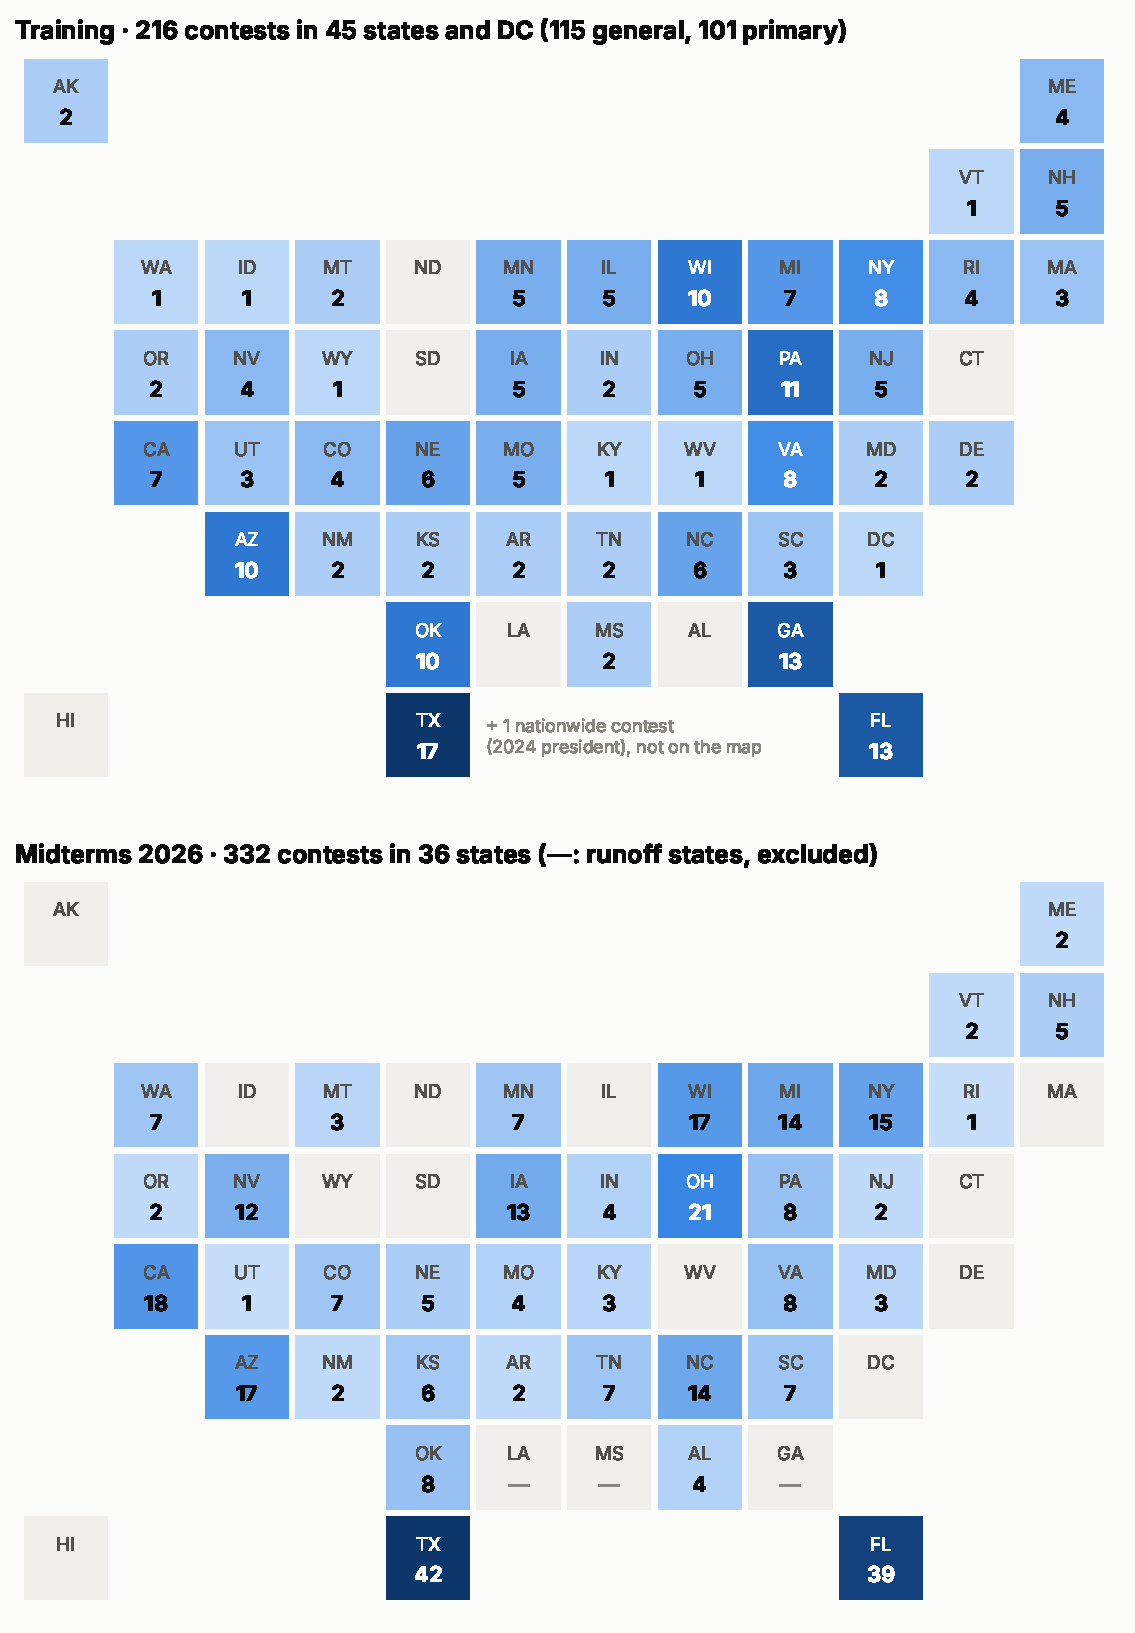
\includegraphics[width=0.78\textwidth]{figures/data_states.pdf}
\caption{Contests per state, both exchanges together. Top: the 216 training contests (general elections and
primaries). Bottom: the 332 contests in the midterm test; Georgia, Louisiana and Mississippi were excluded in advance.
Each map has its own colour scale.}\label{fig:states}
\end{figure}

\begin{figure}[t]
\centering
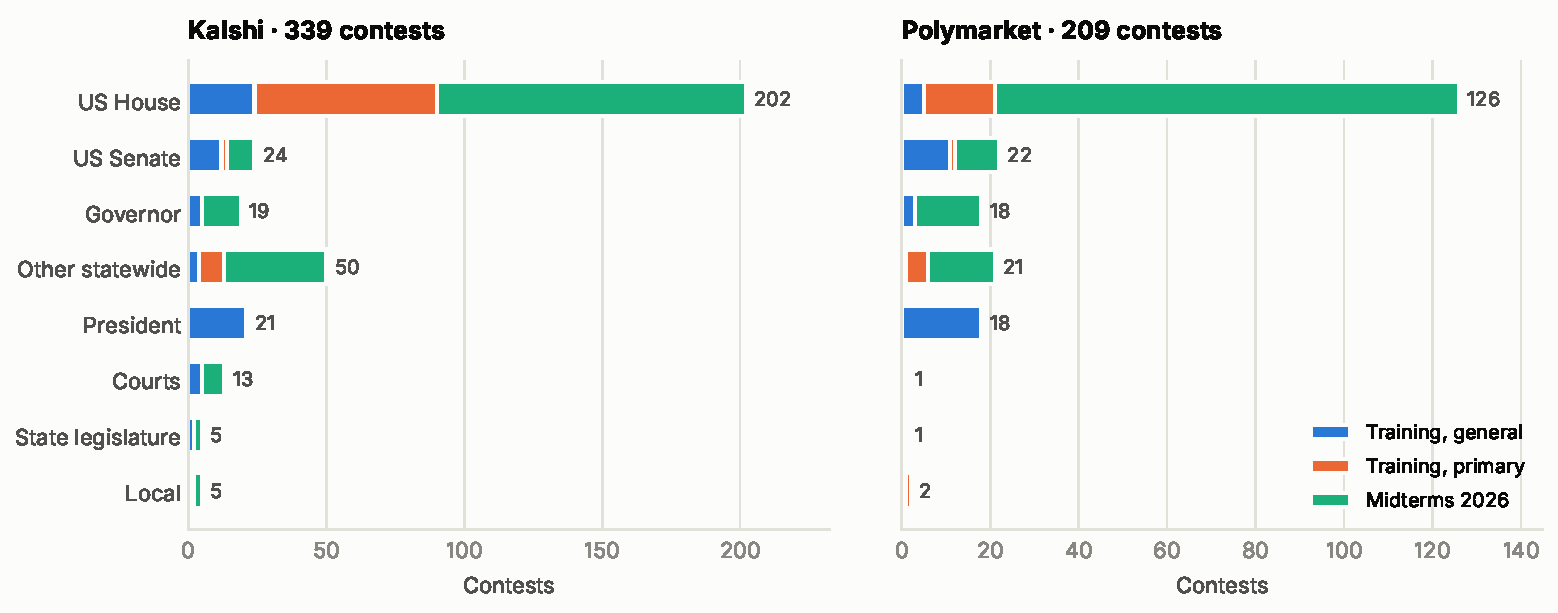
\includegraphics[width=\textwidth]{figures/data_offices.pdf}
\caption{Contests per office on each exchange, split into training general elections, training primaries and the
midterm test.}\label{fig:offices}
\end{figure}

\begin{figure}[t]
\centering
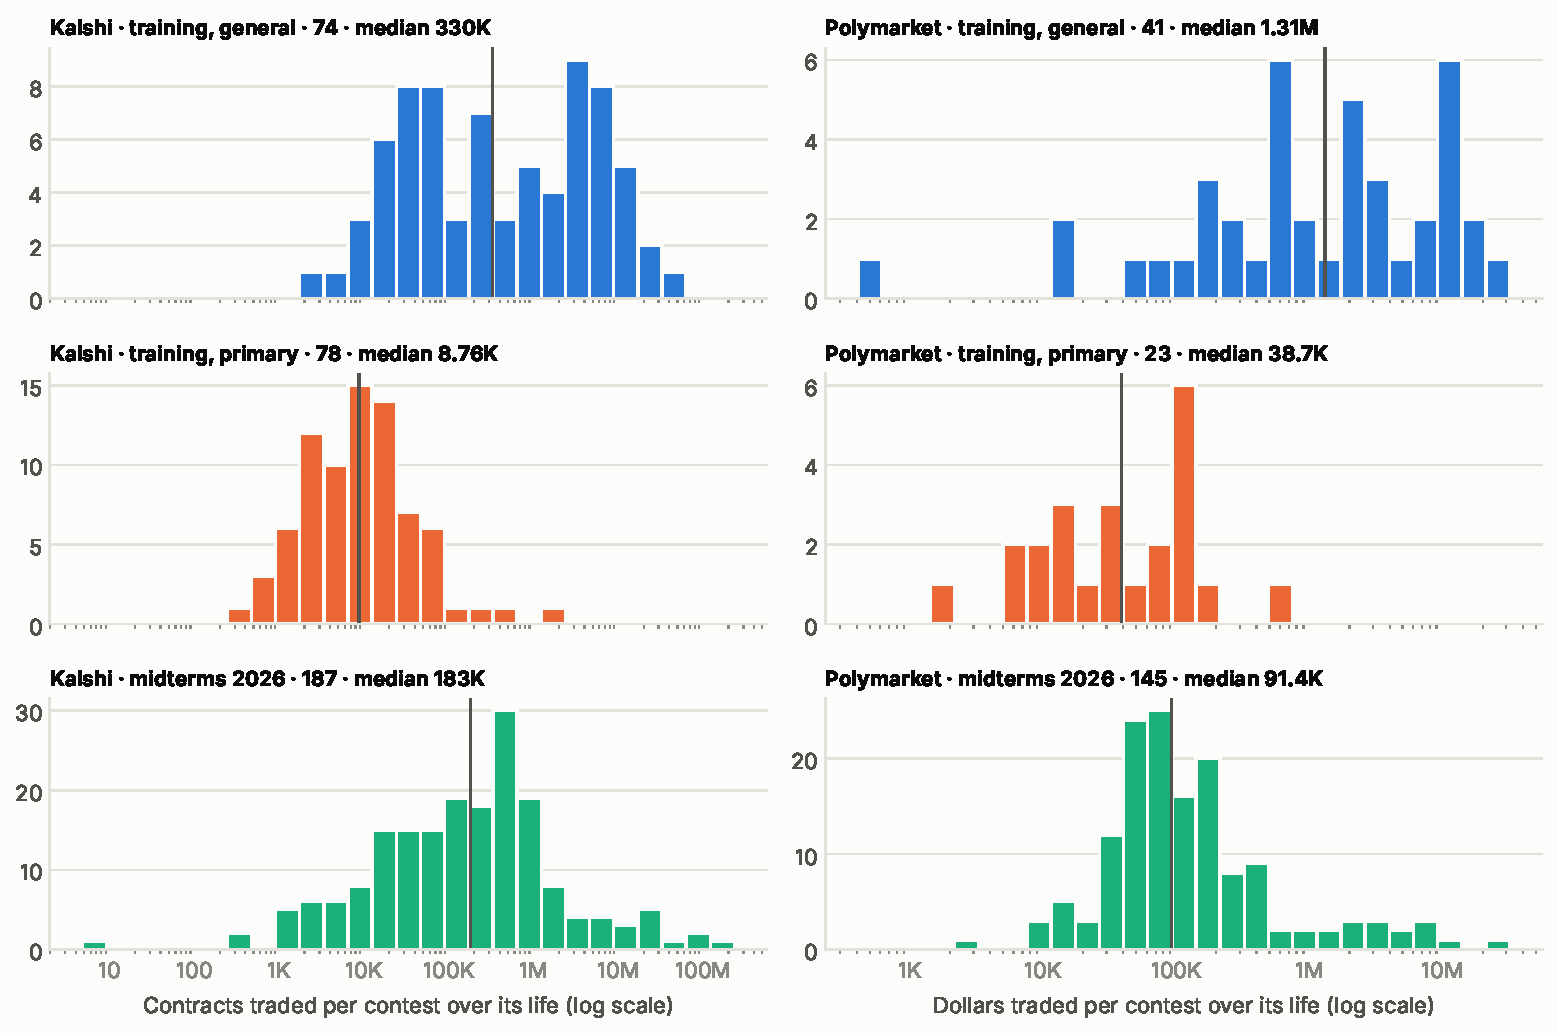
\includegraphics[width=\textwidth]{figures/data_volume.pdf}
\caption{Total volume traded per contest over its life, summed over the two candidate markets, on a log scale. The line
marks the median. Kalshi counts contracts and Polymarket dollars.}\label{fig:volume}
\end{figure}

\begin{figure}[t]
\centering
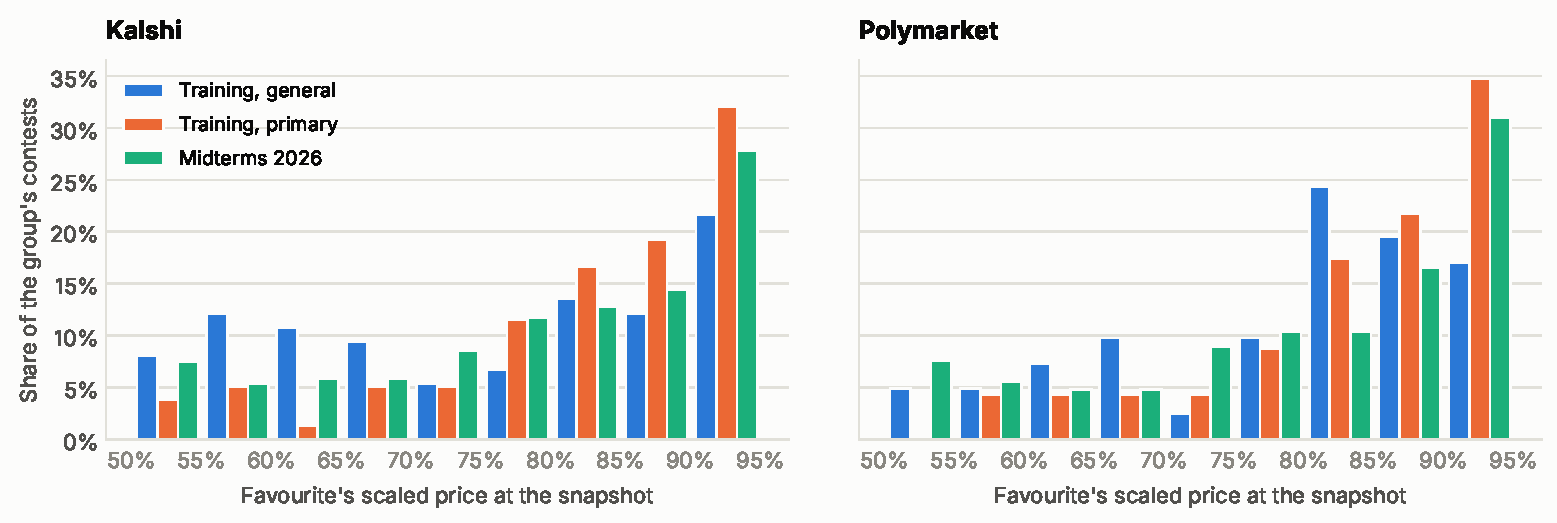
\includegraphics[width=\textwidth]{figures/data_favourites.pdf}
\caption{The favourite's scaled price at the snapshot, as a share of each group's contests. Every analysed contest lies
between 50\% and 95\% by construction.}\label{fig:favourites}
\end{figure}

\section{Method and the pre-registered test}\label{sec:method}

\subsection{The stretch}

Each contest enters once, seen from the favourite's side. Write $p$ for the favourite's scaled price at the snapshot,
between 0.5 and 0.95, and let the favourite either win or lose. The model gives the favourite the chance
\begin{equation}\label{eq:stretch}
  \frac{p^{\,b}}{p^{\,b} + (1-p)^{b}},
\end{equation}
where $b$ is a single number, the \emph{stretch}, shared by every contest in a group. When $b = 1$ the chance equals the
price and the market is calibrated. When $b$ is above 1, the model pushes every price away from 50\%: favourites are
given a higher chance than their price, and the market is \emph{underconfident}. When $b$ is below 1, prices are
pulled towards 50\% and the market is \emph{overconfident}. To give a sense of scale, a stretch of 1.65 turns an 80\%
favourite into a 91\% chance, and a stretch of 0.32 turns it into a 61\% chance.

Equivalently, the stretch multiplies the log-odds of the price: the model's log-odds of a favourite winning are $b$
times $\log\{p/(1-p)\}$. It is therefore a logistic regression of the result on the log-odds of the price with no
intercept, the recalibration slope of \citet{le2026} without its intercept. There is no intercept because the two sides
of a contest are mirror images: the model treats a price of 70\% for one candidate and 30\% for the other the same way
whichever candidate is listed first, so there is no direction in which an intercept could push. We estimate $b$ by
maximum likelihood, the value that gives the actual winners the highest joint chance, using Newton's method. A contest
priced at exactly 50\% says nothing about $b$. When every favourite in a group won, the likelihood keeps rising as $b$
grows and the estimate has no upper limit; we report this as ``no limit'' rather than as a number.

The stretch is deliberately simple. It summarises a whole group of contests with one number that has a direct reading,
it is the correction a forecaster would apply, and it has one parameter to estimate from samples of a few dozen to a
few hundred contests. It assumes that the bias has the same form at every price level, an assumption the calibration
charts in Section~\ref{sec:results} allow the reader to check.

\subsection{Intervals}

Contests are not independent. On a general-election night, a national swing moves races in every state the same way;
within a state, races share voters, polls and polling errors. Treating each contest as an independent draw would make
the estimates look more certain than they are. Every interval in this paper therefore comes from resampling whole
groups of contests: 2{,}000 resamples, drawn with a fixed seed (20261101), each refitting the stretch on the resampled
contests. The 95\% interval runs from the 2.5th to the 97.5th percentile of the 2{,}000 refitted values. When more than
2.5\% of resamples have every favourite winning, the upper end has no limit.

Two resampling units are used. For the training data, which span many election days, the main interval resamples
whole \emph{election days}, so that a night with a common polling miss enters or leaves as one block. For a single
night such as the midterms, days cannot be resampled, and the interval resamples whole \emph{states}. We also report
state-resampled intervals for the training data, so that every group can be compared on the same footing. Resampling
single contests, which ignores both kinds of dependence, is reported only as a reference.

\subsection{The pre-registered test}

The test was written, run on the 2024 data as a check, and archived before the vote. It applies to each platform
separately.

\paragraph{Sample.} US general-election contests voted on 3 November 2026 that are on the list made before the vote,
have settled with one of their two listed candidates winning, and pass every price rule, priced at 22:00 UTC on
3 November. Every office counts. Contests in Georgia, Louisiana and Mississippi are excluded, because a race there can
be decided by a later runoff rather than by the 3 November vote. A platform with fewer than five contests is not
tested.

\paragraph{Two questions.} The test fits the stretch on the midterm sample and computes its 95\% interval by resampling
states. It then asks:
\begin{itemize}
  \item \textbf{Level.} If the whole interval lies above 1, the platform's general-election markets are
        \emph{underconfident}; if it lies below 1, \emph{overconfident}. Otherwise there is \emph{no detectable
        miscalibration}.
  \item \textbf{Change.} The same interval is compared with the platform's stretch on 5 November 2024, fixed in
        advance at 1.972 for Kalshi and 1.828 for Polymarket. If the whole interval lies below that value, the
        stretch is \emph{lower than 2024}; if above it, \emph{higher than 2024}. Otherwise it is \emph{consistent with
        2024}.
\end{itemize}
The 2024 value is treated as a fixed number, not as an estimate with its own interval. This was decided before the vote,
on the basis of a check on the 2024 data: comparing two intervals of this width cannot detect even a large change, and
the question of interest is whether the 2026 markets differ from what was seen in 2024. A stretch with no upper limit is
kept as it is, and the verdicts read only the ends of the interval.

\paragraph{Readings.} The two answers combine into one of four readings, fixed in advance (Table~\ref{tab:readings}).
The first supports the explanation that primaries are traded differently from general elections; the second and third
support, fully or in part, the explanation that the underconfidence of 2024 faded over time.

\begin{table}[t]
\centering\small
\caption{The pre-registered readings of the midterm test, per platform.}\label{tab:readings}
\begin{tabular}{p{4.6cm}p{3.3cm}p{6.2cm}}
\toprule
Level & Change & Reading \\
\midrule
Underconfident & Consistent with or higher than 2024 & Underconfidence persists in general elections: supports ``primaries are traded differently''. \\
No detectable miscalibration, or overconfident & Lower than 2024 & Underconfidence has not persisted: supports ``it switched off over time''. \\
Underconfident & Lower than 2024 & Still underconfident, but less than in 2024: partial support for ``it switched off over time''. \\
Any other combination & & Inconclusive. \\
\bottomrule
\end{tabular}
\end{table}

\paragraph{Stages.} Midterm markets settle over days or weeks, and some only once results are certified. The test
therefore runs twice. A \emph{preliminary} run, allowed from 10 November 2026, uses the contests settled by then and
reports how many listed contests are still open. Races still uncalled are more often those in which the favourite
underperformed, so the preliminary run leans towards finding underconfidence. The \emph{final} run takes place once
every listed contest has settled, or on 31 January 2027, whichever comes first; contests still unsettled then are left
out. The reading is judged on the final run only. This version of the paper reports the preliminary run.

\paragraph{Safeguards.} Before testing, the script recomputes the 2024 stretch for each platform from the price table
and stops if it differs from the frozen value. That guarantees the midterm rows were added without changing any earlier
data. It also stops if any midterm contest is priced at a moment other than the fixed snapshot.

\subsection{What was frozen, and where}

Before 3 November 2026, the complete analysis was made public and archived:
\begin{itemize}
  \item the code, the training results and the midterm test, as release \texttt{v1.0-preregistration} of the public
        repository, archived on Zenodo \citep{kirillov2026code};
  \item the raw market data downloaded from both exchanges, archived separately \citep{kirillov2026data};
  \item a list of SHA-256 fingerprints of the 131 data and result files, so that anyone can check that a later copy
        matches the archived one byte for byte;
  \item the list of midterm contests, made from the open markets before the vote.
\end{itemize}
The test script was run on 5 November 2024 as a self-test and reproduced the frozen 2024 values. Code written after the vote to
download and clean the settled midterm markets, and one change to where Polymarket trades are fetched from, are
described in Section~\ref{sec:limitations}. None of them changes a rule.

\subsection{Analyses beyond the pre-registered test}

The following analyses were not part of the frozen test. They are reported as exploratory, and where they produce
p-values, these are descriptive.

\paragraph{Forecast accuracy.} Prices and stretched prices are scored by their \emph{log loss}, the average of minus
the log of the chance given to what actually happened, and by their \emph{Brier score}, the average squared gap
between the chance and the result; lower is better on both. In the training data, each election day is scored with a
stretch fitted on all the other days. On the midterms, the stretch values are fixed before the vote: the frozen 2024
value, and the values fitted on all earlier general elections, all earlier primaries and all earlier contests. The
improvement is the log loss of the raw prices minus that of the stretched prices, with an interval from resampling
states while the stretch is held fixed. As a reference, the midterms are also scored with their own fitted stretch,
which is the best any single stretch could have done.

\paragraph{Significance.} For the level question, we report the share of state resamples at or below 1, and a test of
the stretch against 1 whose standard error allows for contests in one state moving together. For the accuracy
question, we compare the log loss of raw and stretched prices with a standard error that allows for the same
dependence. Naive versions that treat contests as independent are shown alongside, to make the effect of this
dependence visible.

\paragraph{Same races on both platforms.} The list made before the vote names each race (for example, the House seat
for a given district). Races that both platforms listed and that passed every rule on both are matched by that name,
and the stretch is fitted again on this shared set on each platform. This separates differences in how the platforms
priced the same races from differences in which races they listed.

\paragraph{Other checks.} The training results are recomputed for all countries instead of the US only, and on Kalshi
without the five contests in which neither candidate traded in the day before the snapshot (Polymarket's rules
already exclude such contests; Kalshi's do not). Primaries are split into states with and without runoffs, and by
how long their markets took to settle. The trading backtest is described in Section~\ref{sec:backtest}.

\section{Results}\label{sec:results}

The results come in three parts: the training period, whose numbers were frozen before the vote; the pre-registered
midterm test; and exploratory analyses carried out after the vote. Only the second part is confirmatory.

\subsection{The training period}

\paragraph{General elections are underconfident, Kalshi's primaries are not.}
Table~\ref{tab:training} reports the stretch for every group in the training data. On the general-election night of
5 November 2024, the stretch was 1.97 on Kalshi, with an interval from 1.27 to 3.77 that lies entirely above 1, and 1.83
on Polymarket, with an interval from 0.99 to no upper limit. Across all training general elections, the stretch was 1.28
on Kalshi and 1.61 on Polymarket. These general-election groups span only six or seven election days, and one of them,
5 November 2024, holds most of the contests, so resampling whole days gives very wide intervals; resampling states,
which keeps every day in, gives intervals of 0.83 to 2.62 and 0.80 to no upper limit. Kalshi's 78 primaries point the
other way: a stretch of 0.32, with 99\% of day resamples at or below 1. Polymarket's 23 primaries are close to
calibrated (0.88). Pooling everything, Kalshi's markets look overconfident (0.58, 97\% of resamples at or below 1),
because its primaries outnumber its general elections.

\begin{table}[htbp]
\centering\small\setlength{\tabcolsep}{4.5pt}
\caption{The stretch in the training period, frozen before the vote. Intervals are 95\%; ``no limit'' means enough
resamples had every favourite winning that the stretch has no upper bound. The frozen fitting routine stops at the
wrong value on a few resamples of Kalshi's election days (Section~\ref{sec:limitations}); with a corrected routine,
Kalshi's day-resampled intervals are 0.14 to 1.02 for all contests and 0.01 to 0.69 for primaries, and nothing else in
the table changes.}\label{tab:training}
\begin{tabular}{llrrrll}
\toprule
 & Group & Contests & Days & Stretch & Days resampled & States resampled \\
\midrule
Kalshi & All & 152 & 26 & 0.58 & 0.14 to 1.03 & 0.39 to 0.86 \\
 & General elections & 74 & 6 & 1.28 & $-0.77$ to no limit & 0.83 to 2.62 \\
 & Primaries & 78 & 21 & 0.32 & 0.03 to 0.70 & 0.10 to 0.58 \\
 & 5 November 2024 & 60 & 1 & 1.97 & & 1.27 to 3.77 \\
\midrule
Polymarket & All & 64 & 23 & 1.23 & 0.58 to 1.75 & 0.75 to 2.19 \\
 & General elections & 41 & 7 & 1.61 & 0.33 to no limit & 0.80 to no limit \\
 & Primaries & 23 & 17 & 0.88 & 0.40 to 1.67 & 0.40 to 1.56 \\
 & 5 November 2024 & 35 & 1 & 1.83 & & 0.99 to no limit \\
\bottomrule
\end{tabular}
\end{table}

Figure~\ref{fig:train_calibration} shows the same results as calibration charts. Contests are grouped by the
favourite's price; each dot is the share of favourites that won, and the curve is the fitted stretch. In general
elections the dots sit on or above the diagonal, and every favourite priced above 90\% won. In Kalshi's primaries, the
dots sit well below it: favourites priced between 70\% and 90\% won barely more than half the time.
Figure~\ref{fig:train_stretch} shows the stretch with both kinds of interval, and the distribution of the resampled
stretch for all contests together.

\begin{figure}[tbp]
\centering
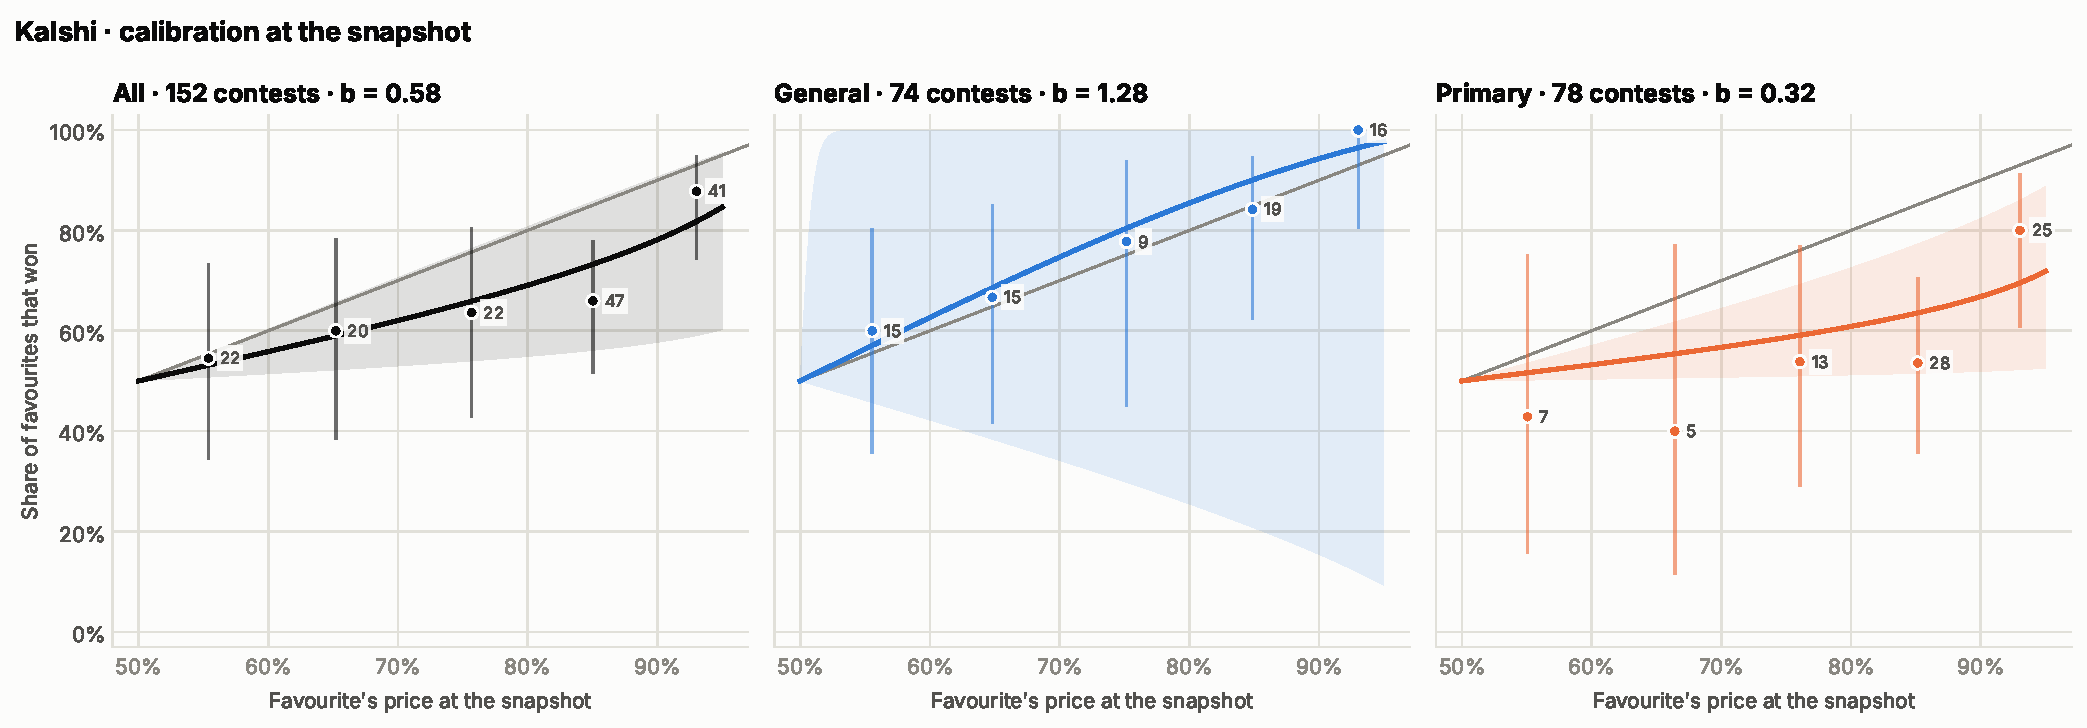
\includegraphics[width=\textwidth]{figures/fit_kalshi_calibration.pdf}\par\medskip
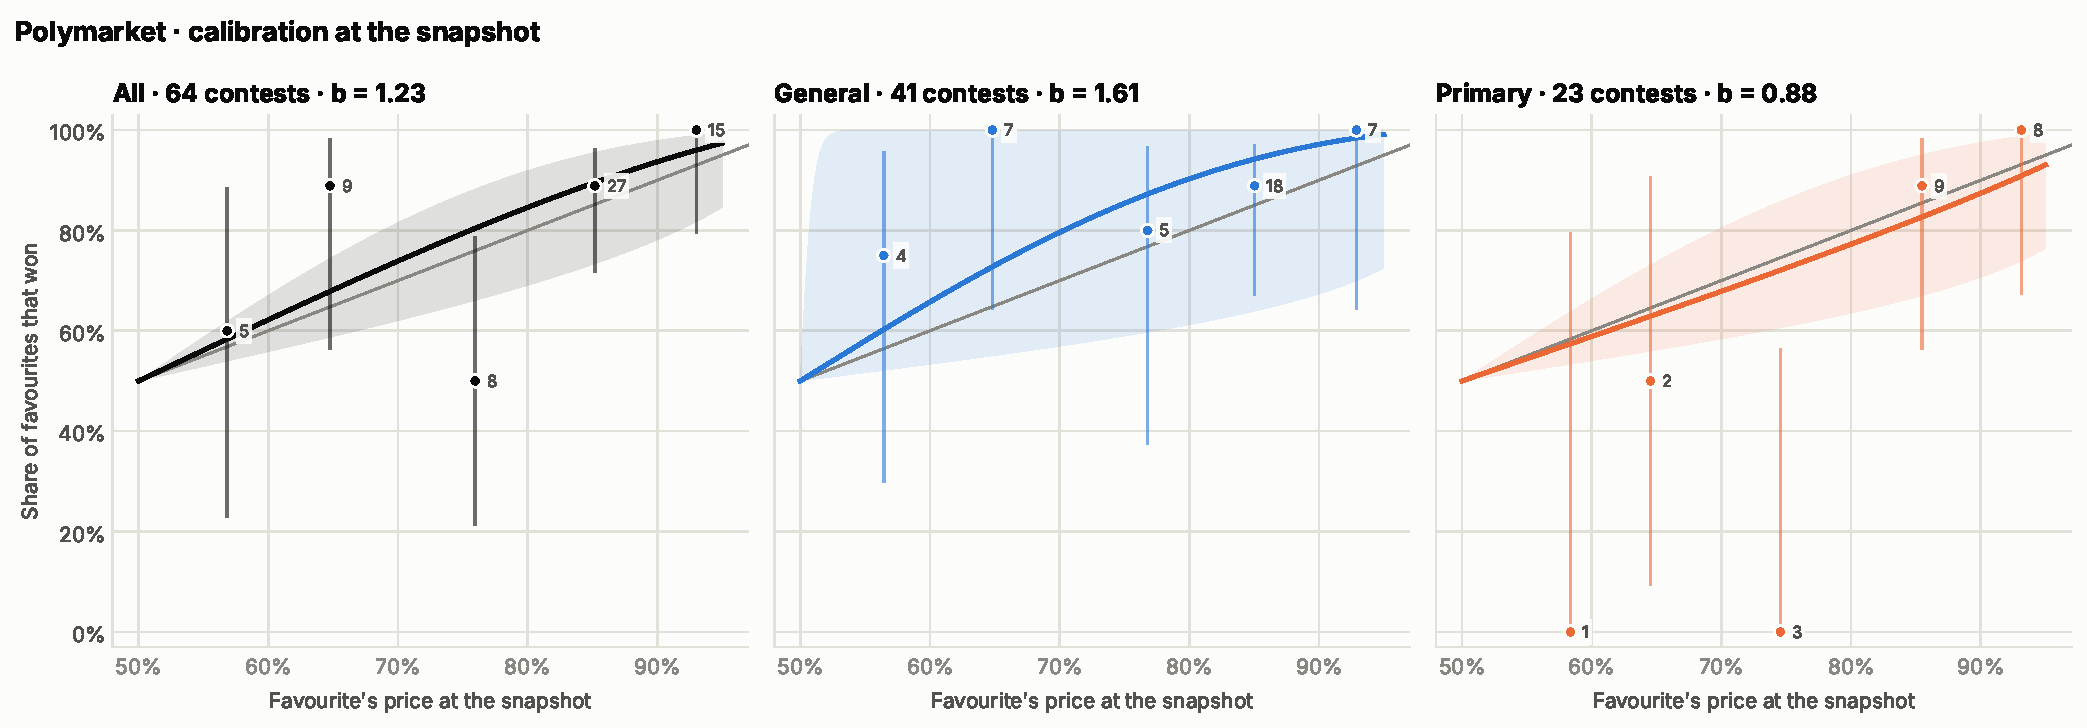
\includegraphics[width=\textwidth]{figures/fit_polymarket_calibration.pdf}
\caption{Calibration in the training period. Dots: share of favourites that won in each price group, with 95\%
intervals and the number of contests. Curve: the fitted stretch, with the range covered by its interval shaded. Grey
diagonal: a calibrated market.}\label{fig:train_calibration}
\end{figure}

\begin{figure}[tbp]
\centering
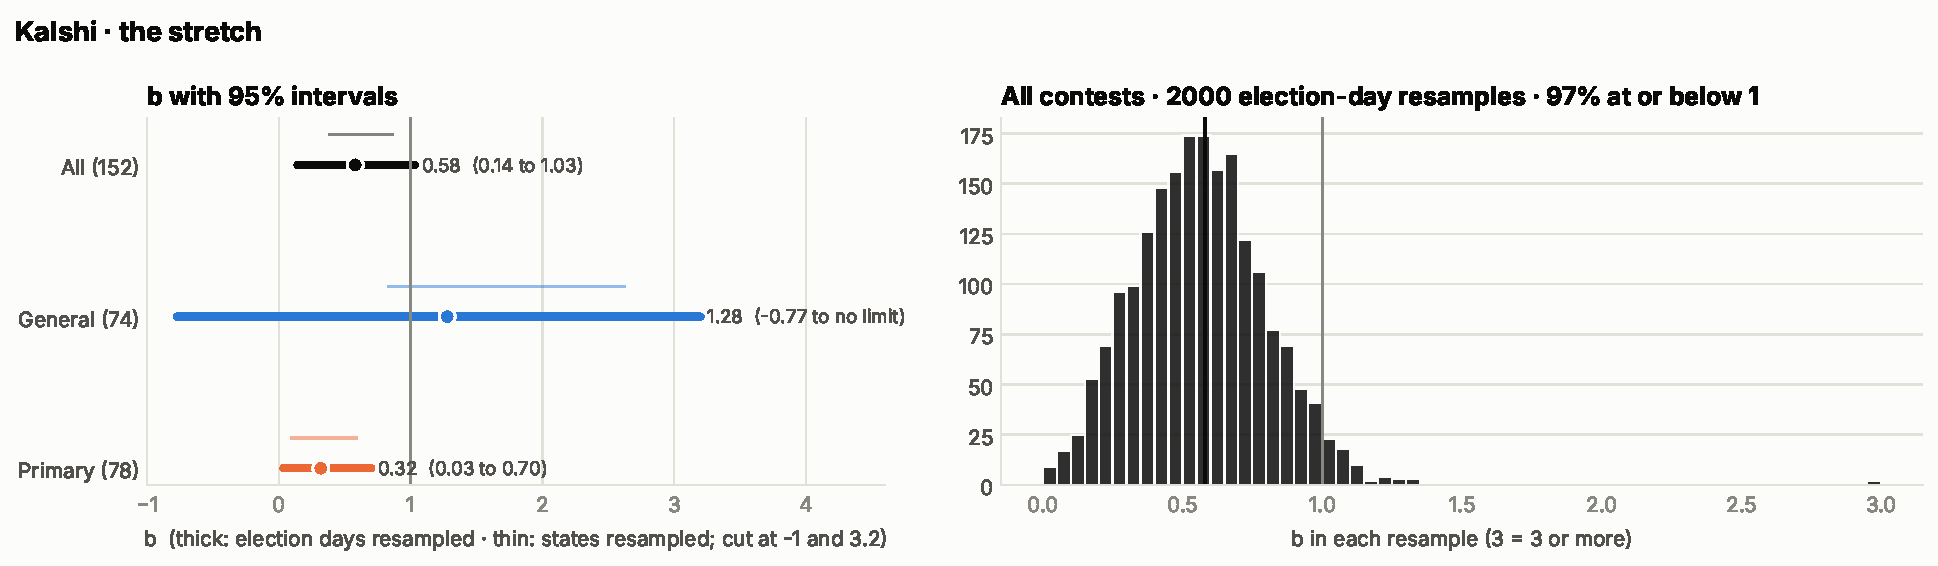
\includegraphics[width=\textwidth]{figures/fit_kalshi_stretch.pdf}\par\medskip
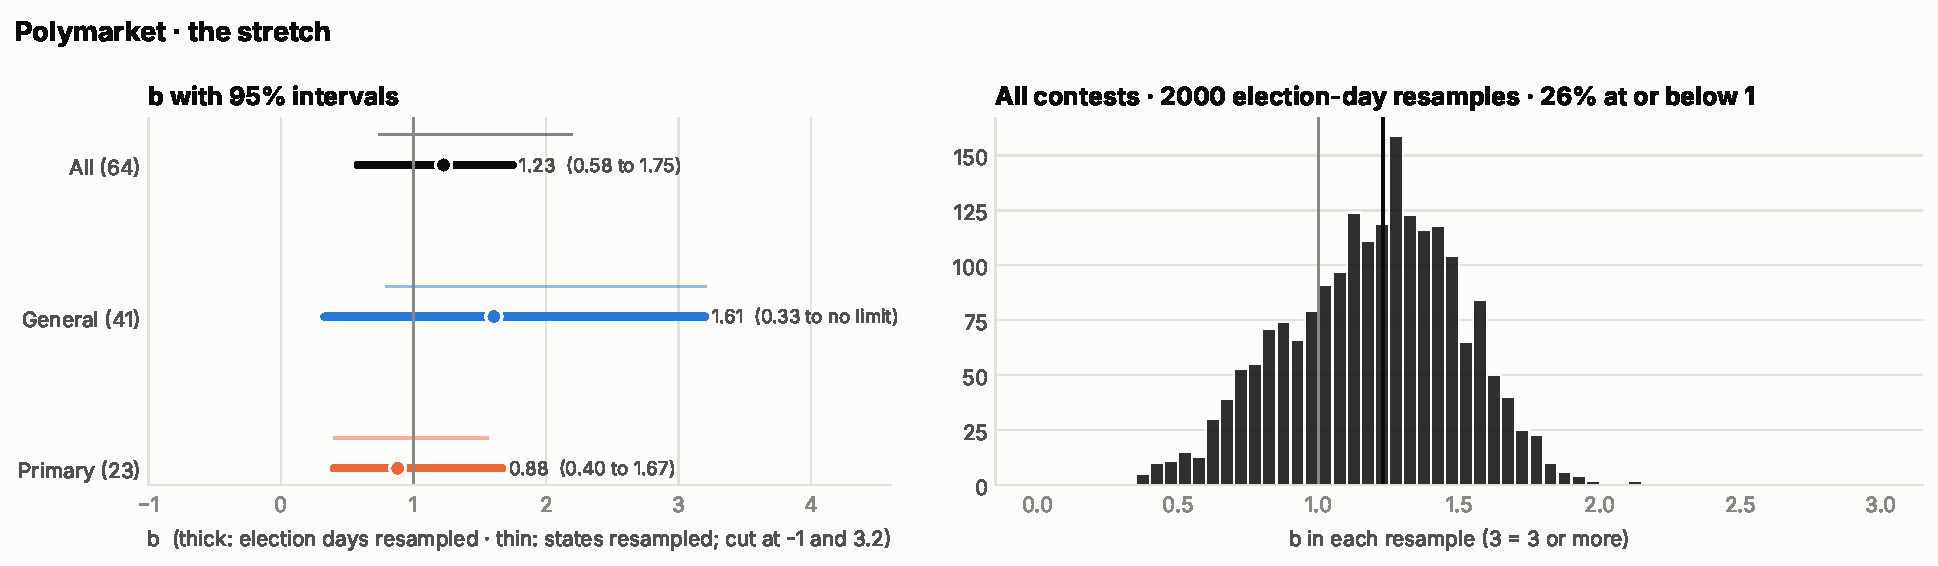
\includegraphics[width=\textwidth]{figures/fit_polymarket_stretch.pdf}
\caption{The stretch in the training period. Left: each group with its interval from resampling election days (thick)
and states (thin). Right: the stretch for all contests, refitted on each of 2,000 resamples of election
days.}\label{fig:train_stretch}
\end{figure}

\paragraph{Robustness.}
No single primary day drives the results (Figure~\ref{fig:lodo}). Leaving out any one election day other than
5 November 2024 keeps Kalshi's overall stretch between 0.53 and 0.69, and Polymarket's between 1.21 and 1.38. Leaving
out 5 November 2024, the night that carries the general-election underconfidence, pulls them down to 0.36 and 0.91.
The same figure shows what happens when one stretch is used for everything. Fitted on all other days and applied to the day left
out, a single stretch barely improves Kalshi's forecasts (log loss 0.001 lower over all contests, better on 14 of 26
days) and worsens Polymarket's (0.025 higher, despite helping on 16 of 23 days). This is what one would expect if the
correction points one way in general elections and the other way in primaries. Adding the contests from other
countries changes little on Kalshi and pulls Polymarket's general-election stretch from 1.61 to 1.15
(Figure~\ref{fig:us_all}). Dropping the five Kalshi contests in which neither candidate traded in the day before the
snapshot gives 0.60, 1.27 and 0.33 for all contests, general elections and primaries.

Kalshi's primary result is also not explained by runoffs (Figure~\ref{fig:primary_checks}). Several upsets were in
states where a primary can go to a runoff, so a market priced on the first round's election day might settle only weeks
later. But outside those states, favourites still lost 16 times where the prices implied 7 (stretch 0.40, 0.03 to
0.83), and 74 of the 78 markets settled within two weeks of the vote (0.33, $-0.01$ to 0.72). In the runoff states the
overconfidence is stronger still: 15 upsets where the prices implied 7 (0.16, $-0.19$ to 1.10). These intervals refit
the stretch with the corrected routine mentioned under Table~\ref{tab:training}.

\begin{figure}[tbp]
\centering
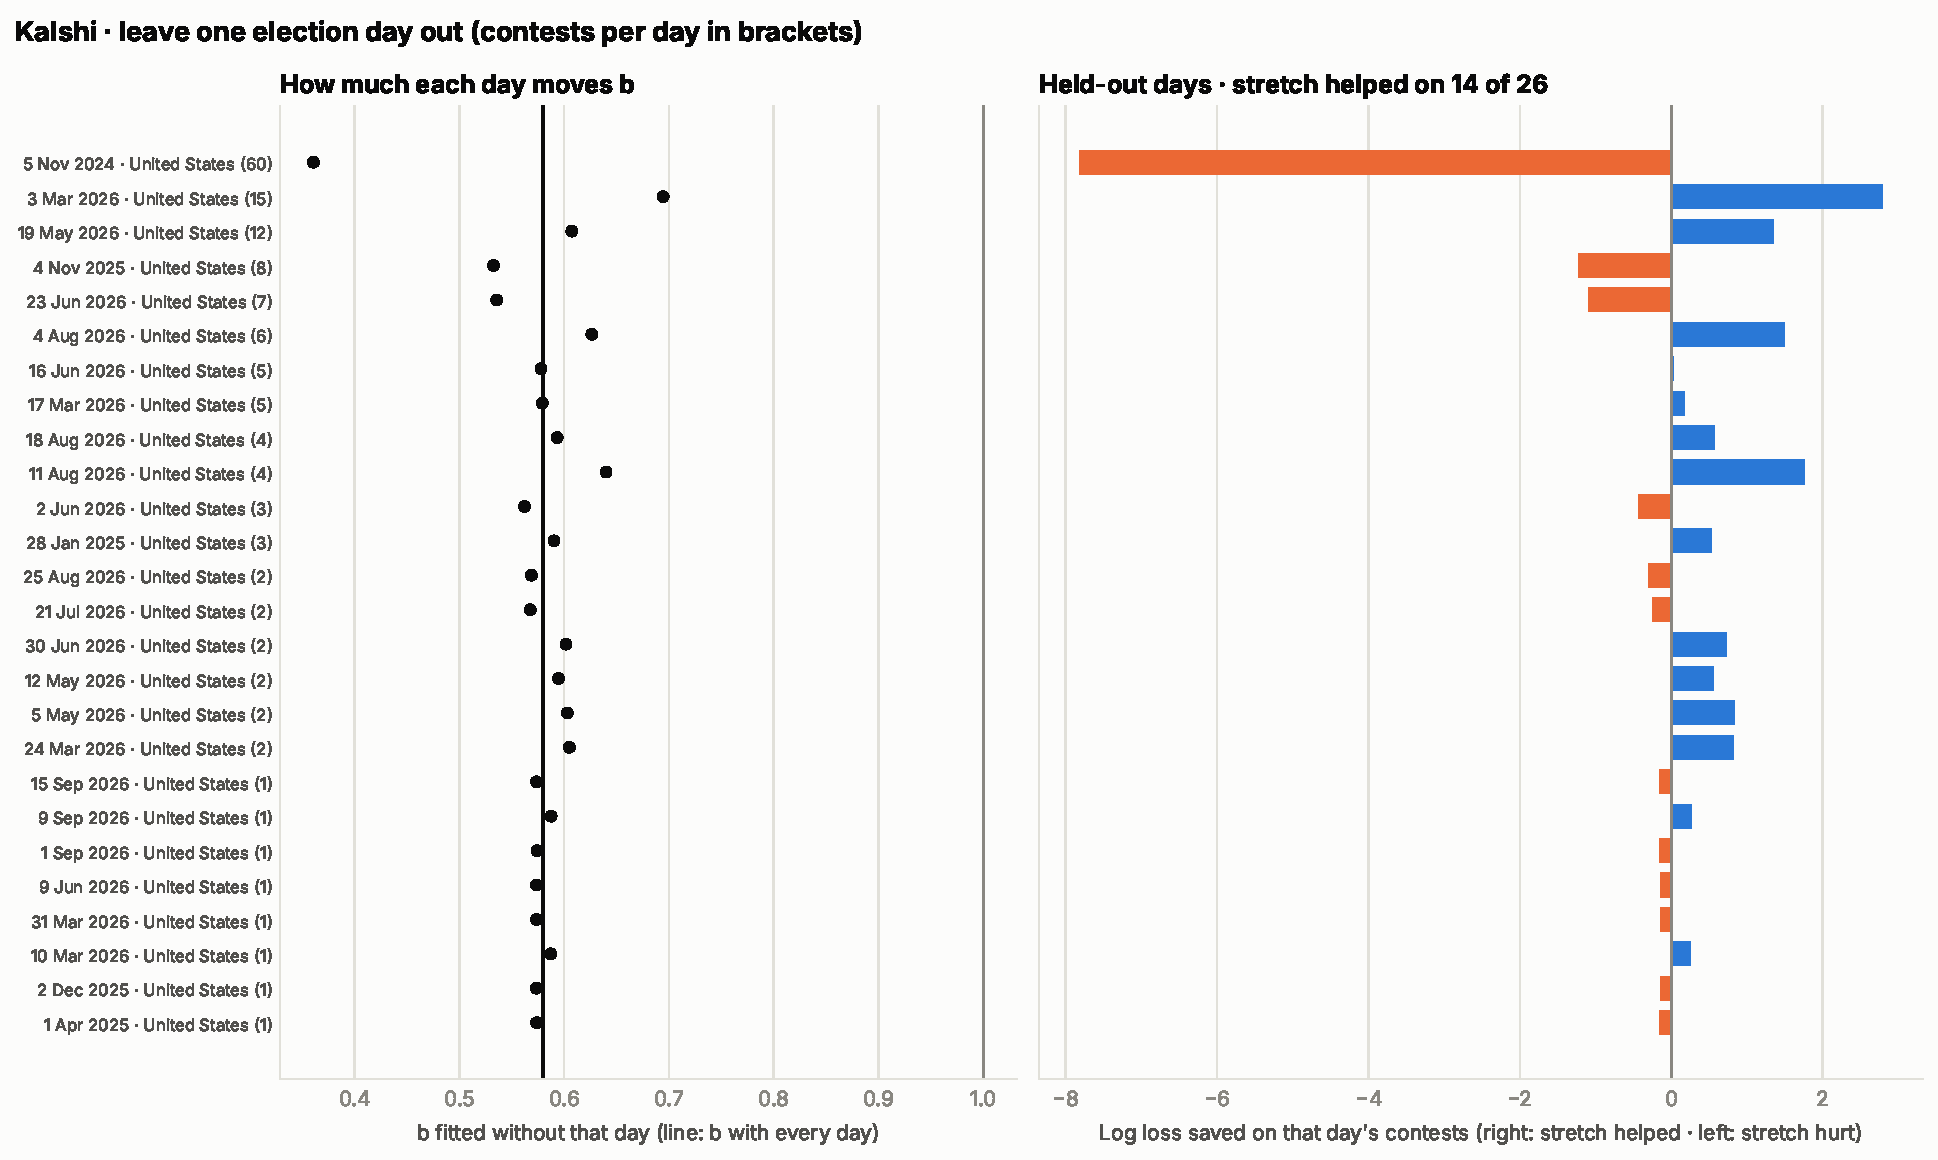
\includegraphics[width=0.92\textwidth]{figures/fit_kalshi_leave_one_day_out.pdf}\par\medskip
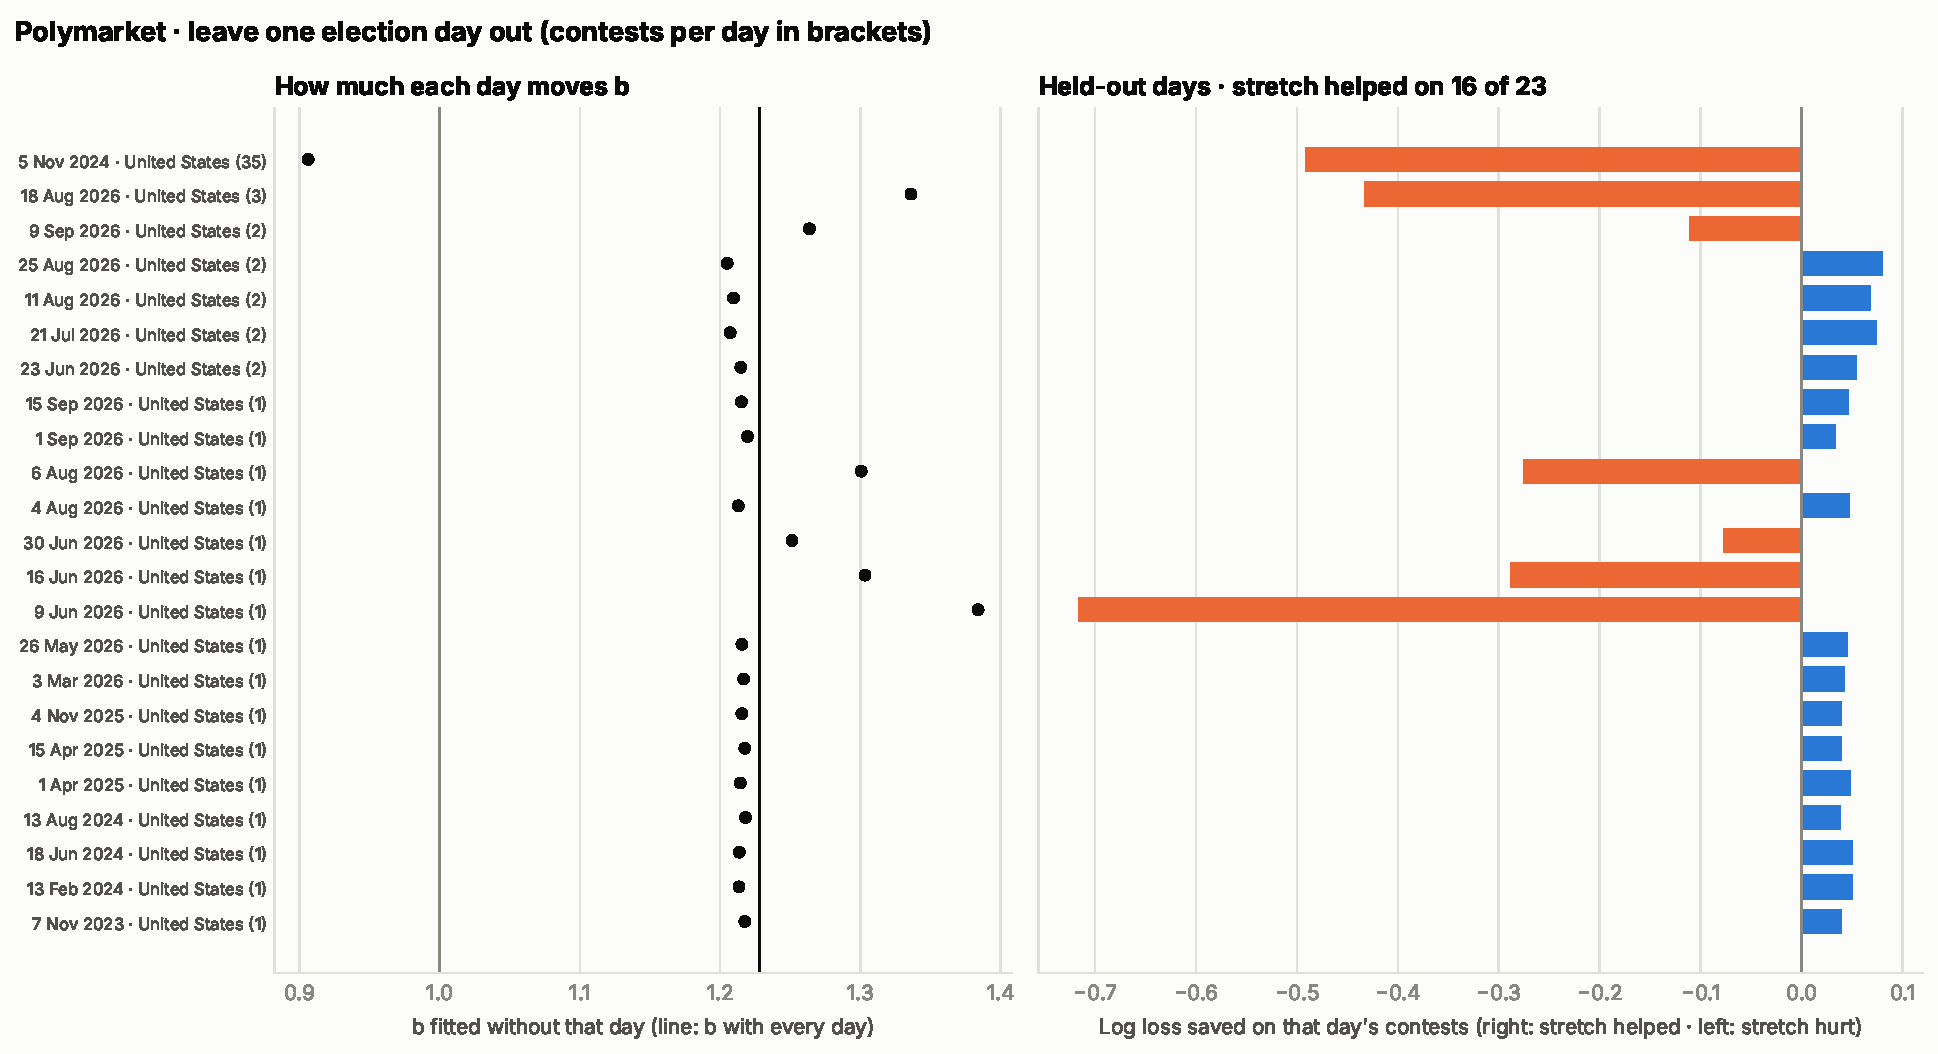
\includegraphics[width=0.92\textwidth]{figures/fit_polymarket_leave_one_day_out.pdf}
\caption{Leaving out one election day at a time. Left: the stretch fitted without that day; the line is the stretch with
every day. Right: how much a stretch fitted on all other days improved (blue) or worsened (orange) the log loss of that
day's contests.}\label{fig:lodo}
\end{figure}

\begin{figure}[tbp]
\centering
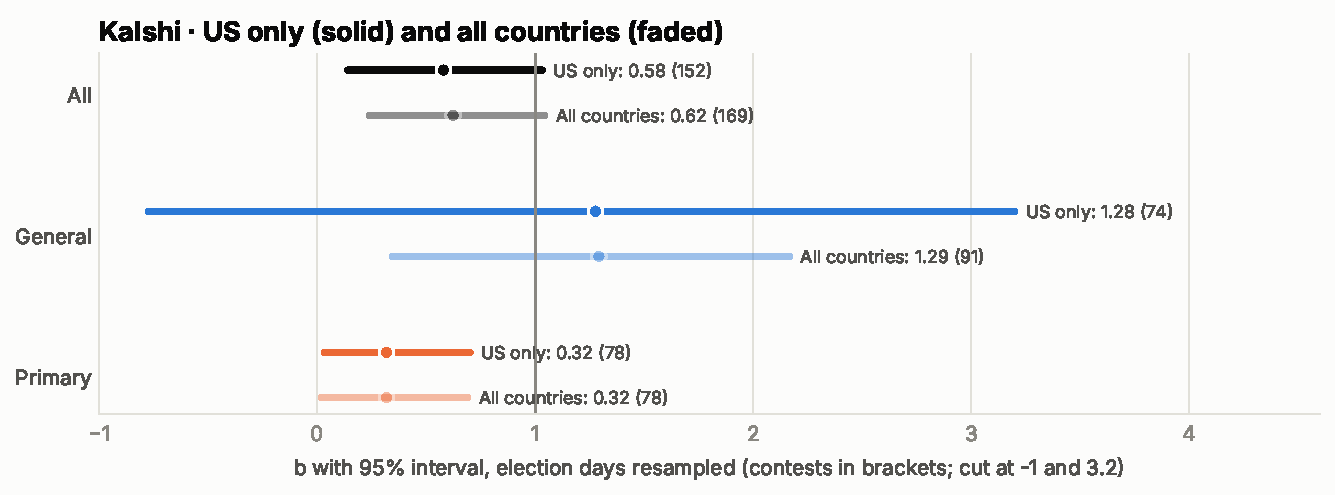
\includegraphics[width=0.85\textwidth]{figures/fit_kalshi_us_vs_all.pdf}\par\medskip
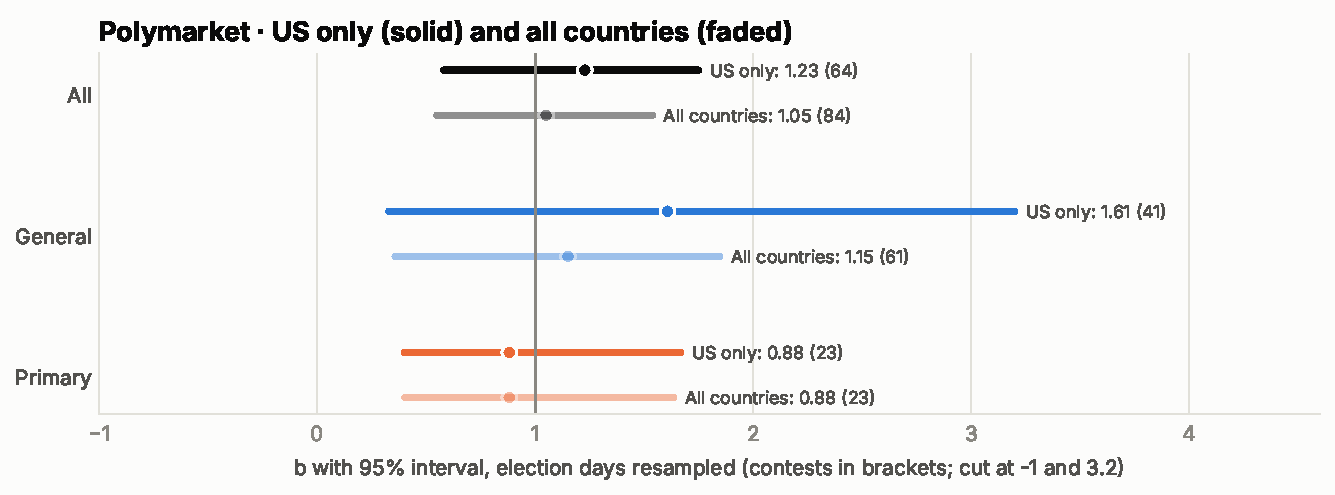
\includegraphics[width=0.85\textwidth]{figures/fit_polymarket_us_vs_all.pdf}
\caption{US contests only (solid) against contests in every country (faded), with intervals from resampling election
days.}\label{fig:us_all}
\end{figure}

\begin{figure}[tbp]
\centering
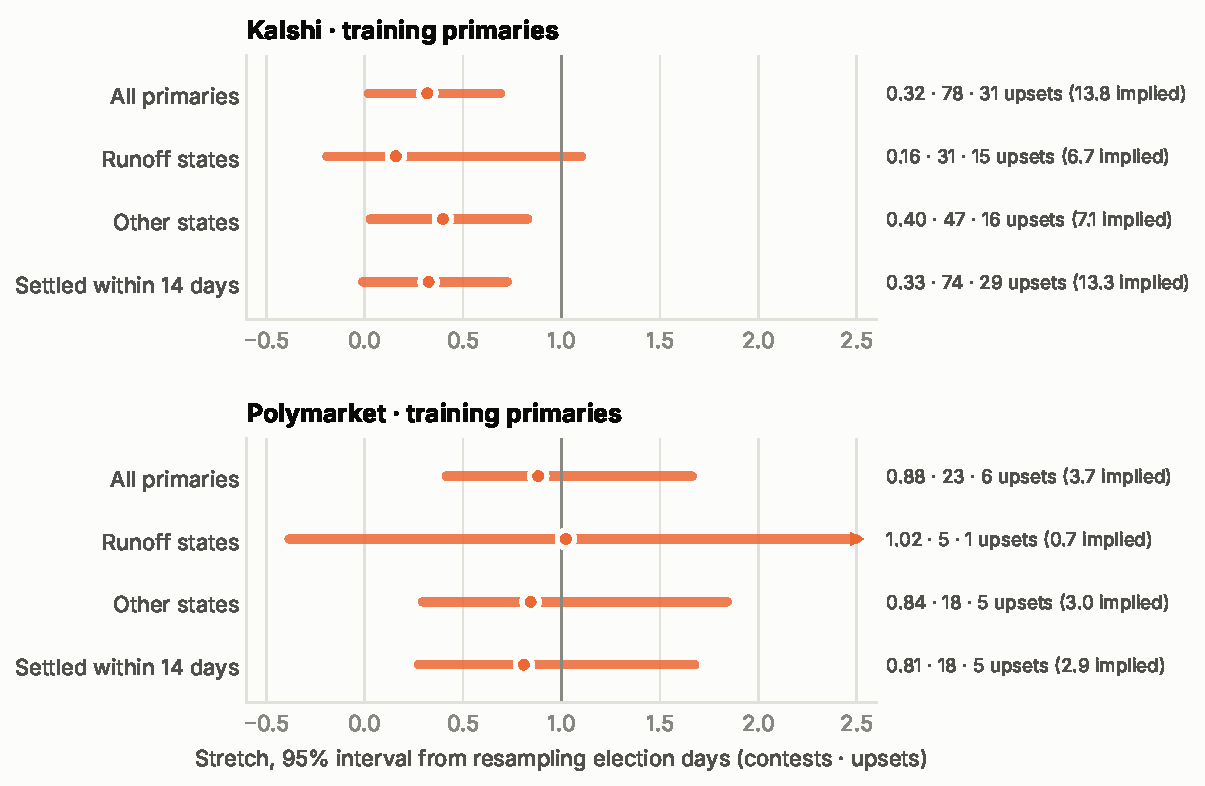
\includegraphics[width=0.85\textwidth]{figures/res_primary_checks.pdf}
\caption{Checks on the training primaries: states where a primary can go to a runoff, other states, and markets that
settled within 14 days of the vote. Intervals resample the primaries' election days, refitting with the corrected
routine, so the first row differs slightly from Table~\ref{tab:training}; arrows mark intervals that run past the edge.
Labels give the stretch, the number of contests, and the upsets against the number the prices
implied.}\label{fig:primary_checks}
\end{figure}

\subsection{The pre-registered midterm test}

Table~\ref{tab:test} reports the preliminary run of the test, on the contests settled by 10 November 2026.
On Polymarket, the stretch of the 145 midterm contests was 1.66, with an interval from 1.21 to 2.91. The whole interval
lies above 1, so Polymarket's general-election markets were \emph{underconfident}, and it includes the 2024 value of
1.83, so they were \emph{consistent with 2024}. The pre-registered reading is that underconfidence persists in general
elections, which supports the explanation that primaries are traded differently. On Kalshi, the stretch of the 187
contests was 1.32, with an interval from 0.88 to 2.35. It includes 1, so there is no detectable miscalibration, and it
includes the 2024 value of 1.97, so it is also consistent with 2024. The pre-registered reading is \emph{inconclusive}.

\begin{table}[htbp]
\centering\small\setlength{\tabcolsep}{4.5pt}
\caption{The pre-registered midterm test, preliminary run of 10 November 2026. Intervals resample states. Forty listed
contests had not yet settled.}\label{tab:test}
\begin{tabular}{lL{1.5cm}L{2.1cm}L{2.5cm}L{2.4cm}L{3.1cm}}
\toprule
 & Contests (states) & Stretch (95\% interval) & Level & Change & Reading \\
\midrule
Kalshi & 187 (36) & 1.32\newline (0.88 to 2.35) & No detectable miscalibration & Consistent with 2024 (1.97) & Inconclusive \\
\addlinespace
Polymarket & 145 (34) & 1.66\newline (1.21 to 2.91) & Underconfident & Consistent with 2024 (1.83) & Underconfidence persists in general elections \\
\bottomrule
\end{tabular}
\end{table}

Figure~\ref{fig:test} draws the test itself. Each panel is the distribution of the stretch over the 2,000 resamples of
states, the same resamples the test used. On Polymarket, all but 4 of the 2{,}000 lie above 1. On Kalshi, 92\% do,
short of the 97.5\% that an interval wholly above 1 requires. Figure~\ref{fig:cmp_stretch} places the midterm values next to every training
group. On both platforms the midterms sit with the earlier general elections and far from the earlier primaries.

\begin{figure}[tbp]
\centering
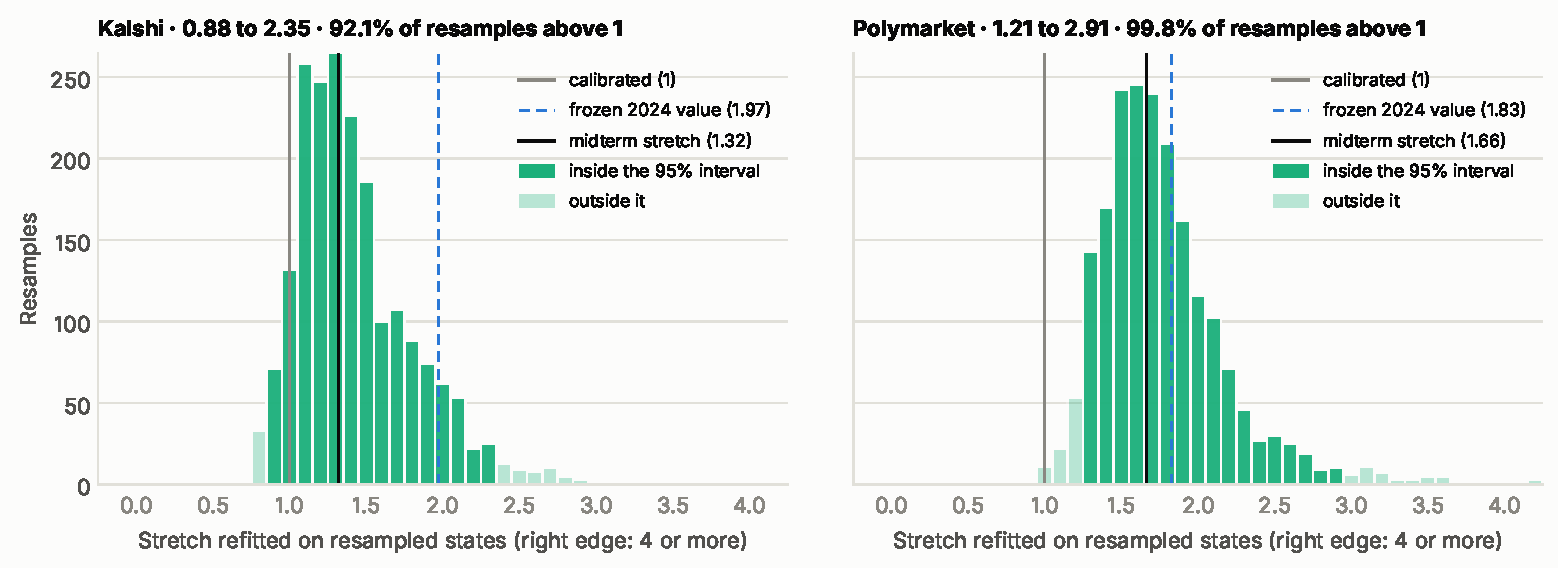
\includegraphics[width=\textwidth]{figures/res_test_resamples.pdf}
\caption{The pre-registered test. The stretch refitted on each of 2,000 resamples of states; the darker bars are the
central 95\%, which is the test's interval. Grey: a calibrated market. Dashed blue: the frozen 2024 value. Black: the
midterm stretch.}\label{fig:test}
\end{figure}

\begin{figure}[tbp]
\centering
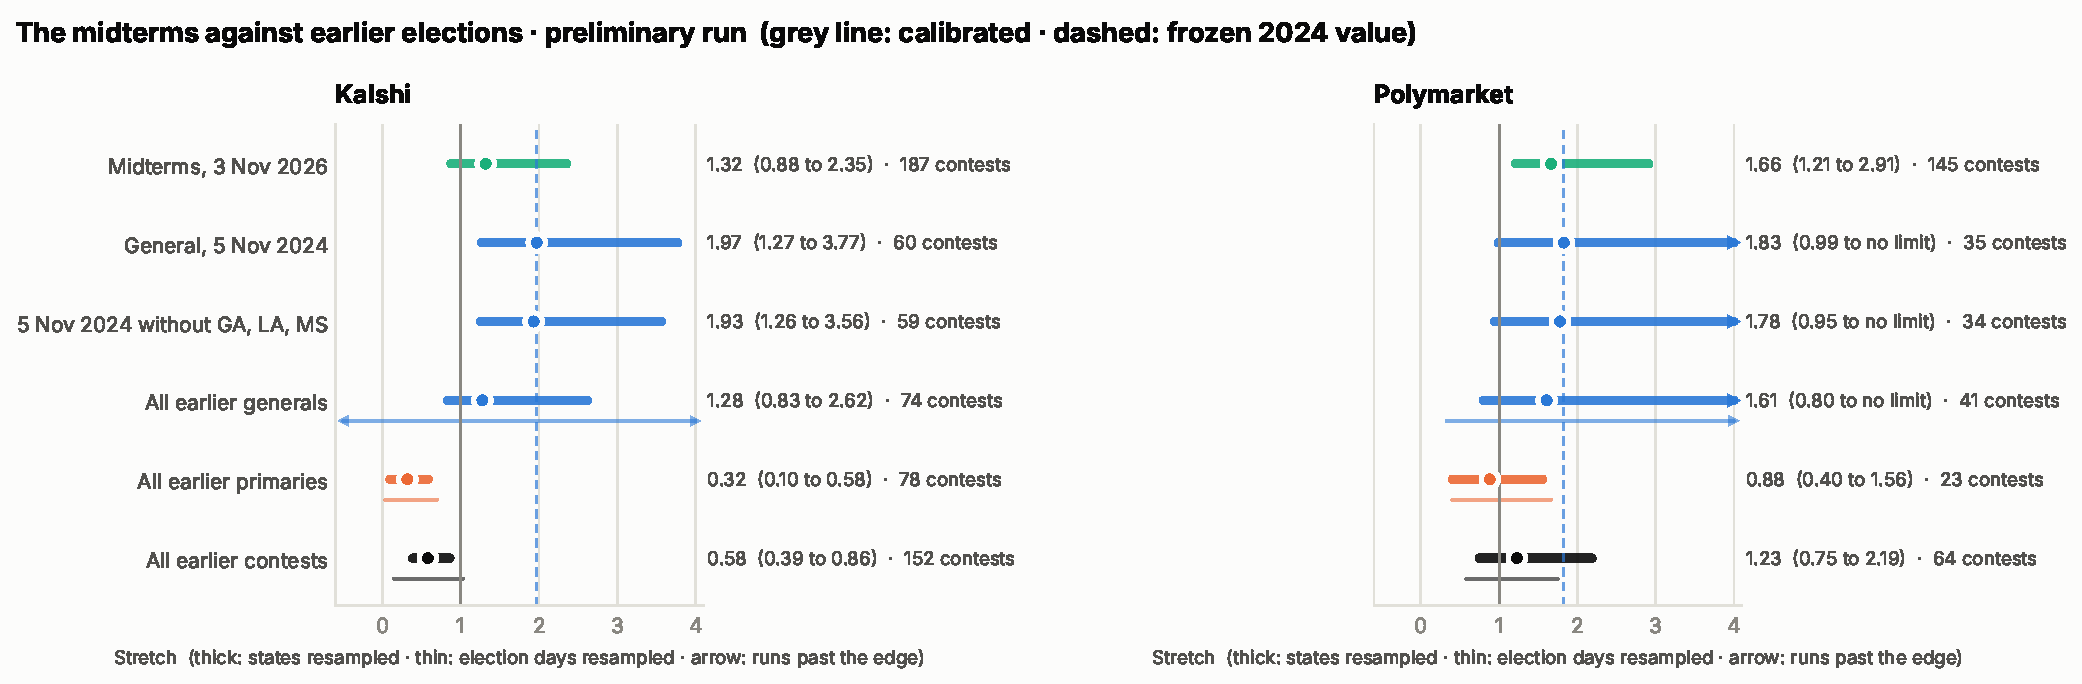
\includegraphics[width=\textwidth]{figures/cmp_stretch.pdf}
\caption{The midterms against the training groups. Thick bars resample states; thin bars, for groups spanning several
election days, resample days. Grey line: a calibrated market. Dashed line: the frozen 2024 value.}\label{fig:cmp_stretch}
\end{figure}

\subsection{Exploratory analyses}\label{sec:exploratory}

Everything in this subsection was examined after the vote. The p-values reported here are descriptive, and several
comparisons were made, so a single result near the 5\% level should be read with caution.

\paragraph{Favourites priced above 80\% almost never lost.}
Figure~\ref{fig:cmp_calibration} compares the midterms with the 2024 night and the earlier primaries, price group by
price group. Midterm favourites priced between 80\% and 95\% won 99 of 104 contests on Kalshi and 83 of 84 on
Polymarket, against average prices of about 85\% to 93\%. Close races were priced about right or slightly too
confidently: favourites priced between 50\% and 70\% won 52\% of the time on Kalshi and 58\% on Polymarket, against an
average price of about 60\%. The underconfidence therefore sits in clear favourites, not in tossups. In all, prices
implied 39 upsets on Kalshi and 29 on Polymarket; there were 35 and 20.

\begin{figure}[tbp]
\centering
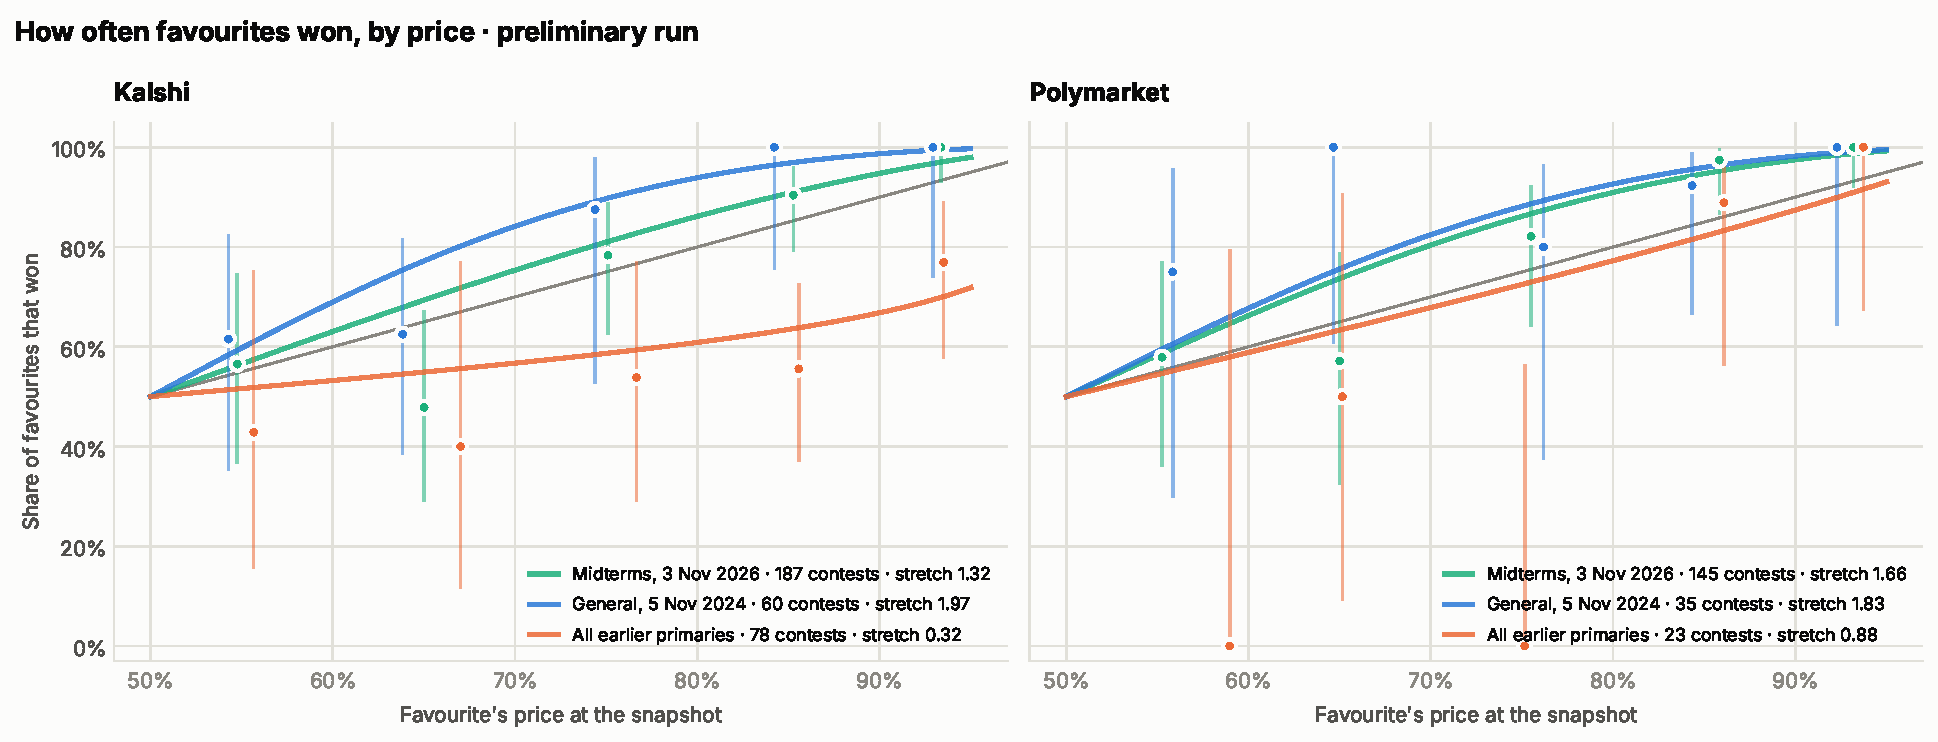
\includegraphics[width=\textwidth]{figures/cmp_calibration.pdf}
\caption{How often favourites won, by price: the midterms (green), the 2024 night (blue) and the training primaries
(orange). Dots: share of favourites that won in each price group, with 95\% intervals. Lines: each group's fitted
stretch. Grey diagonal: a calibrated market.}\label{fig:cmp_calibration}
\end{figure}

\paragraph{Every general-election night looks alike.}
Figure~\ref{fig:cmp_days} shows each election day with at least five contests: how many points more often favourites
won than their average price implied. On the midterms, the gap was $+2.0$ points on Kalshi and $+6.1$ on Polymarket.
On 5 November 2024 it was $+6.8$ and $+12.7$, and on Kalshi's eight contests of 4 November 2025, every favourite won, a gap of
$+13.7$. Of the six Kalshi days that include primaries, four lie below zero, two of them by more than 40 points;
Polymarket has no primary day with five contests.

\begin{figure}[tbp]
\centering
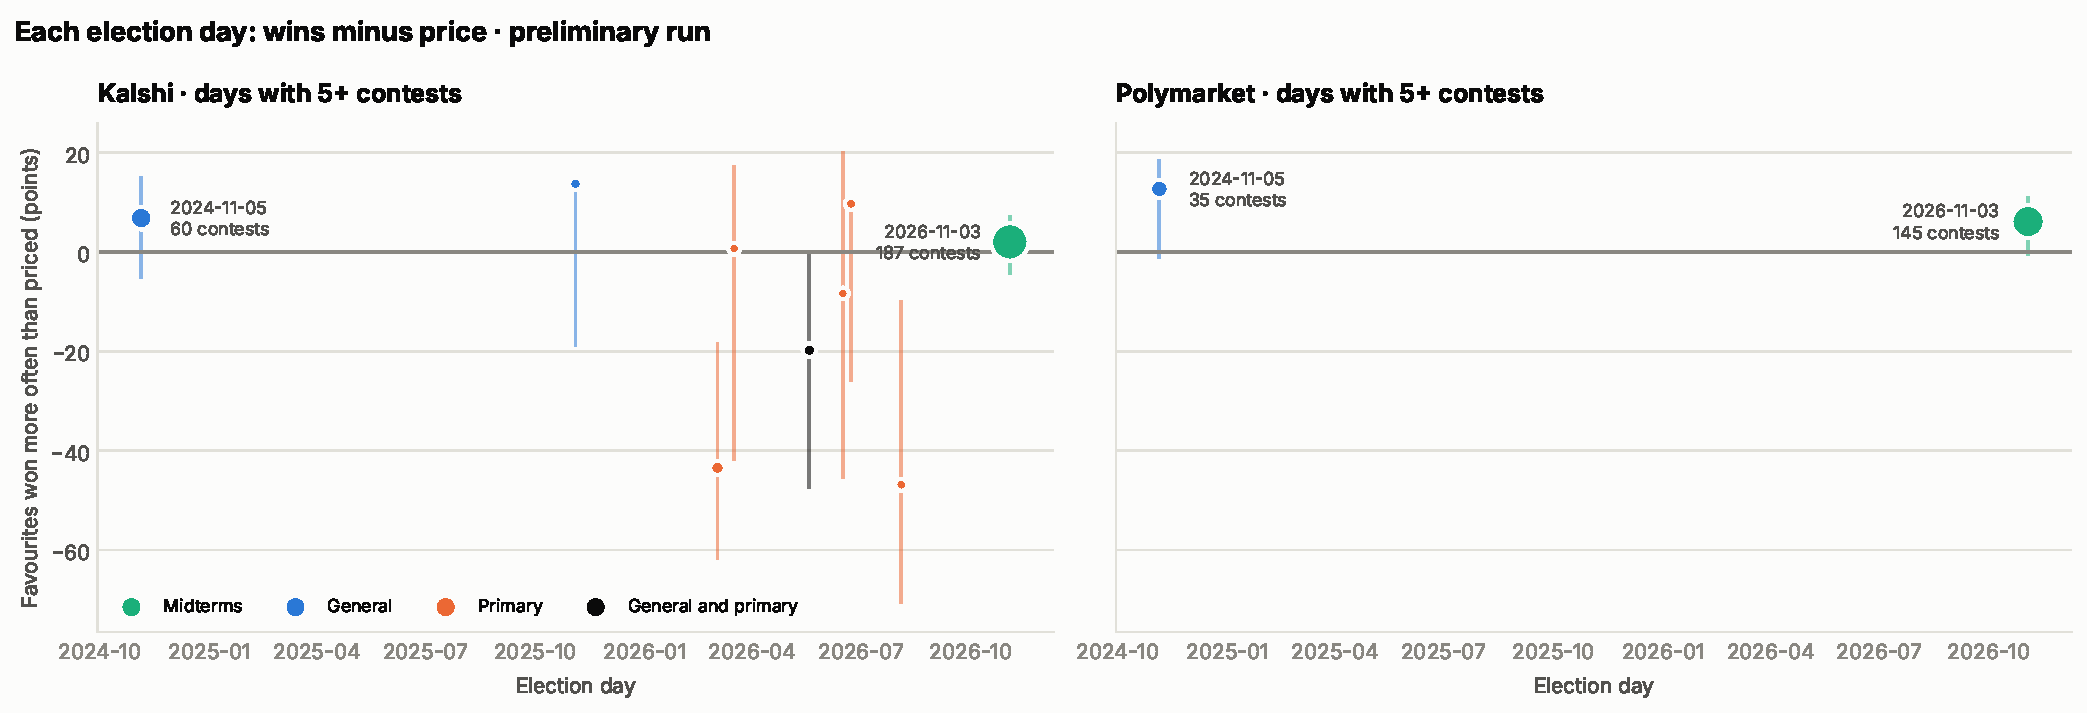
\includegraphics[width=\textwidth]{figures/cmp_election_days.pdf}
\caption{Each election day with at least five contests: share of favourites that won minus their average price, in
percentage points, with a 95\% interval. Dot size: number of contests. Above zero, favourites won more often than
priced.}\label{fig:cmp_days}
\end{figure}

\paragraph{Upsets cluster by state.}
Figure~\ref{fig:upsets} shows where the midterm upsets fell. On Kalshi, Texas alone had 12 upsets where the prices
implied 5, and North Carolina 4 where they implied 1.5; Florida had 1 where they implied 4.2. Polymarket shows the same
places, more mildly. This clustering is why every interval resamples whole states: the 187 Kalshi contests carry closer
to 36 states' worth of independent information than to 187 contests' worth.

\begin{figure}[tbp]
\centering
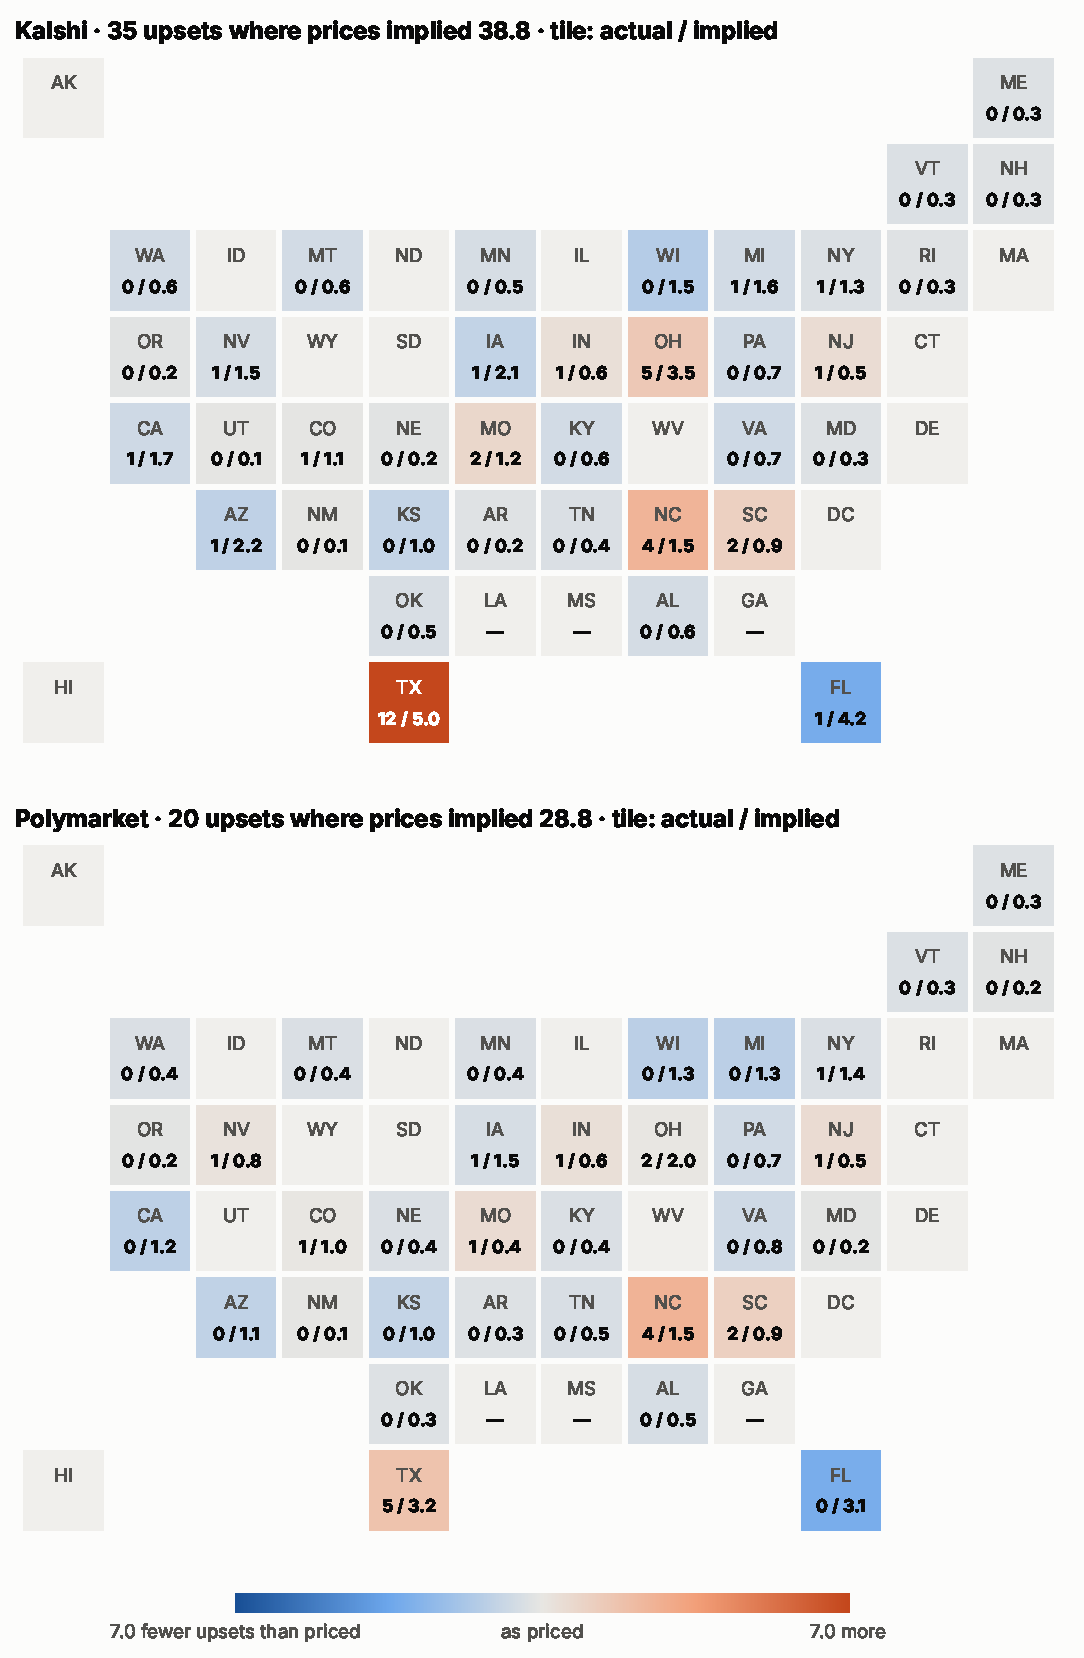
\includegraphics[width=0.74\textwidth]{figures/res_upsets_map.pdf}
\caption{Midterm upsets by state: the number of favourites that lost, against the number the prices implied (the sum of
one minus the favourite's price). Blue: fewer upsets than priced. Orange: more. Georgia, Louisiana and Mississippi were
excluded in advance.}\label{fig:upsets}
\end{figure}

\paragraph{On the same races, the two platforms agree.}
Kalshi's weaker result does not come from pricing races differently. On the 141 races that both platforms listed and
that passed every rule on both, the two had the same favourite every time, and their chances for the eventual winner
differed by 0.9 percentage points on average (Figure~\ref{fig:same_scatter}). On these shared races, both platforms were
underconfident: 1.68 on Kalshi (1.21 to 3.00) and 1.65 on Polymarket (1.18 to 2.89), with 20 upsets each where the
prices implied about 29 (Figure~\ref{fig:same_split}). The difference lies in the 46 races that only Kalshi listed: mostly down-ballot statewide offices such as
treasurer and attorney general, eight state supreme court seats, three mayors and three state legislative seats, with
nine House seats. There, favourites lost 15 times where the prices implied 10, a stretch of 0.75 (0.38 to 2.04). Six of
the 15 upsets were supreme court seats in Texas and Ohio. Resampling states jointly, Kalshi's overall stretch minus Polymarket's is $-0.34$, with
an interval from $-0.79$ to $0.09$: Kalshi came out lower in 91\% of resamples, but the difference is not significant.
The training data show a similar pattern on a much smaller scale. Kalshi's 14 general-election contests outside the
2024 night had 4 upsets where the prices implied 2, all in low-profile 2026 races: two Florida legislative special
elections and two Georgia Supreme Court seats. If the prices had been right, four or more upsets would have occurred
14\% of the time.

\begin{figure}[tbp]
\centering
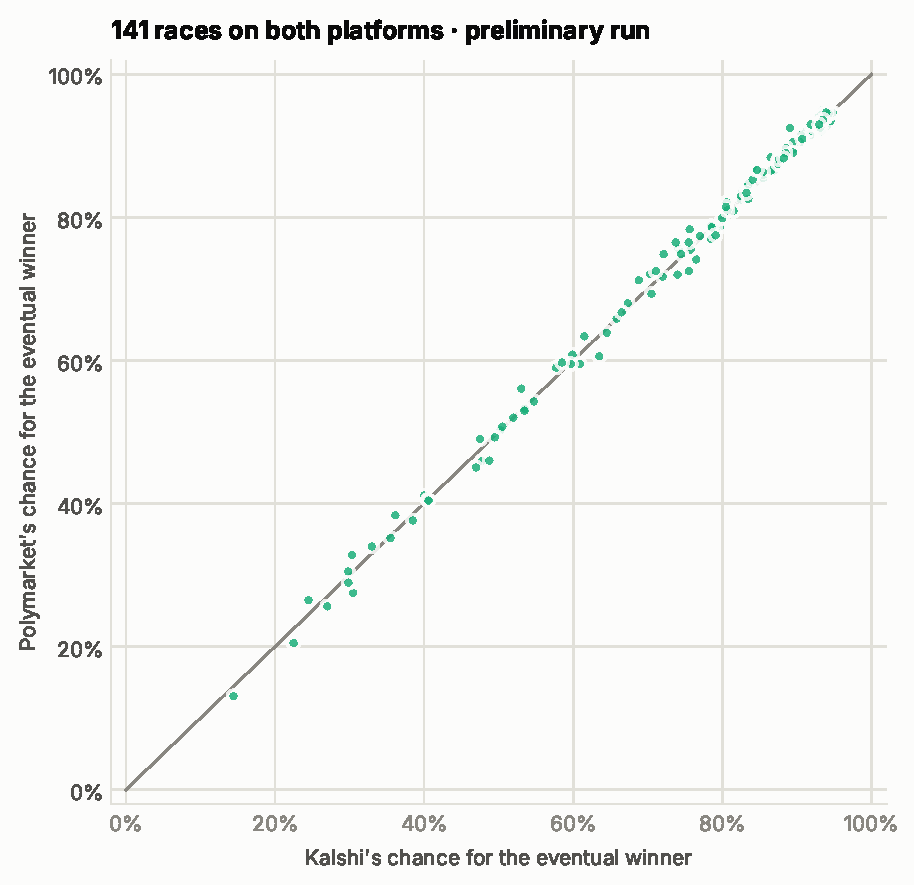
\includegraphics[width=0.5\textwidth]{figures/cmp_same_races.pdf}
\caption{The 141 midterm races on both platforms: the chance each gave the candidate who won. Dots above the diagonal
mean Polymarket gave the winner more.}\label{fig:same_scatter}
\end{figure}

\begin{figure}[tbp]
\centering
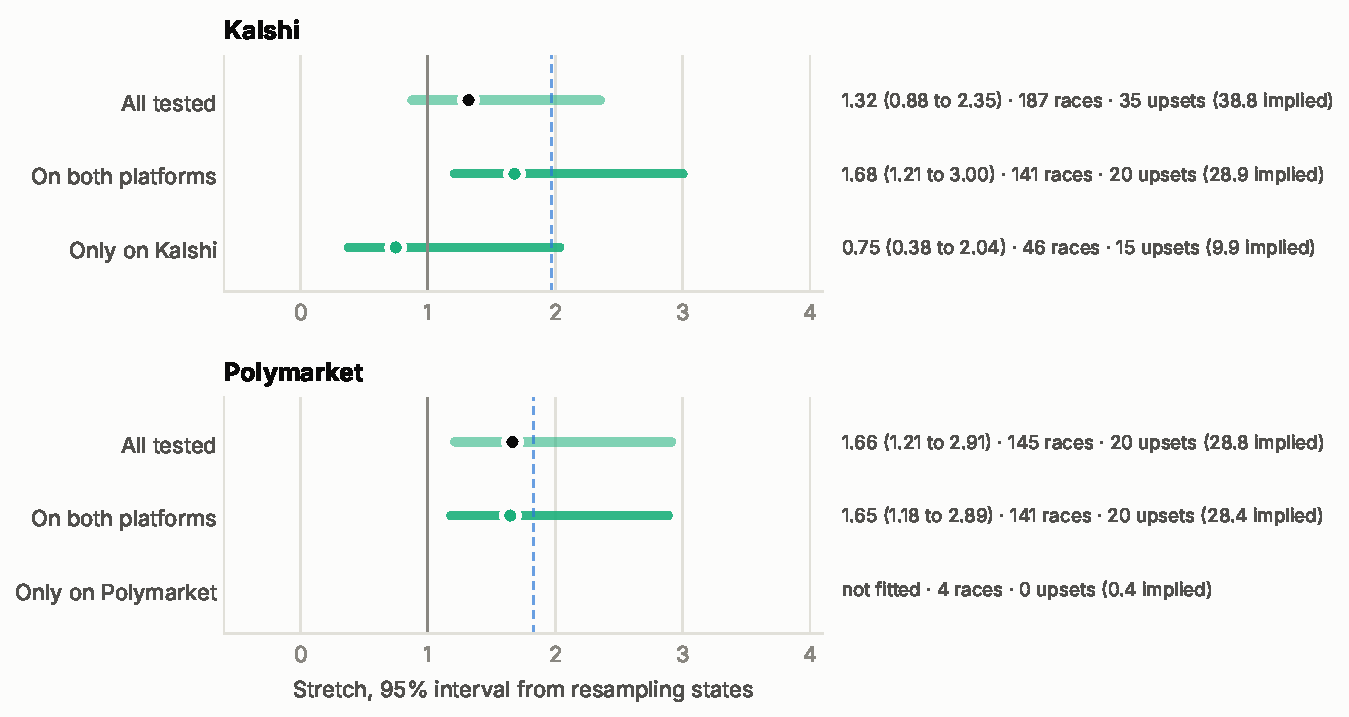
\includegraphics[width=0.92\textwidth]{figures/res_same_races.pdf}
\caption{Each platform's midterm contests split into races on both platforms and races on that platform only.
Intervals resample states. Grey line: a calibrated market. Dashed line: the frozen 2024 value. Polymarket listed only
four races that Kalshi did not, too few to fit.}\label{fig:same_split}
\end{figure}

\paragraph{Would the earlier stretch have improved the midterm prices?}
Applying a stretch fixed before the vote to the midterm prices tests the correction out of sample
(Figure~\ref{fig:scores}). On Polymarket, every value learned from general elections improved the log loss by close to
the most any single stretch could have: the frozen 2024 value by 0.032 ($-0.027$ to 0.081), the value from all earlier
general elections by 0.033 ($-0.010$ to 0.069), against a ceiling of 0.033. On Kalshi, the earlier general-election
value improved it slightly (0.010, $-0.020$ to 0.036, equal to the ceiling), while the 2024 value overcorrected and
made it slightly worse ($-0.017$). Values learned from primaries made the prices clearly worse on both platforms: by
0.143 on Kalshi and 0.016 on Polymarket, with intervals that exclude zero. A correction learned from general elections
carries over to the next general election; one learned from primaries does not.

\begin{figure}[tbp]
\centering
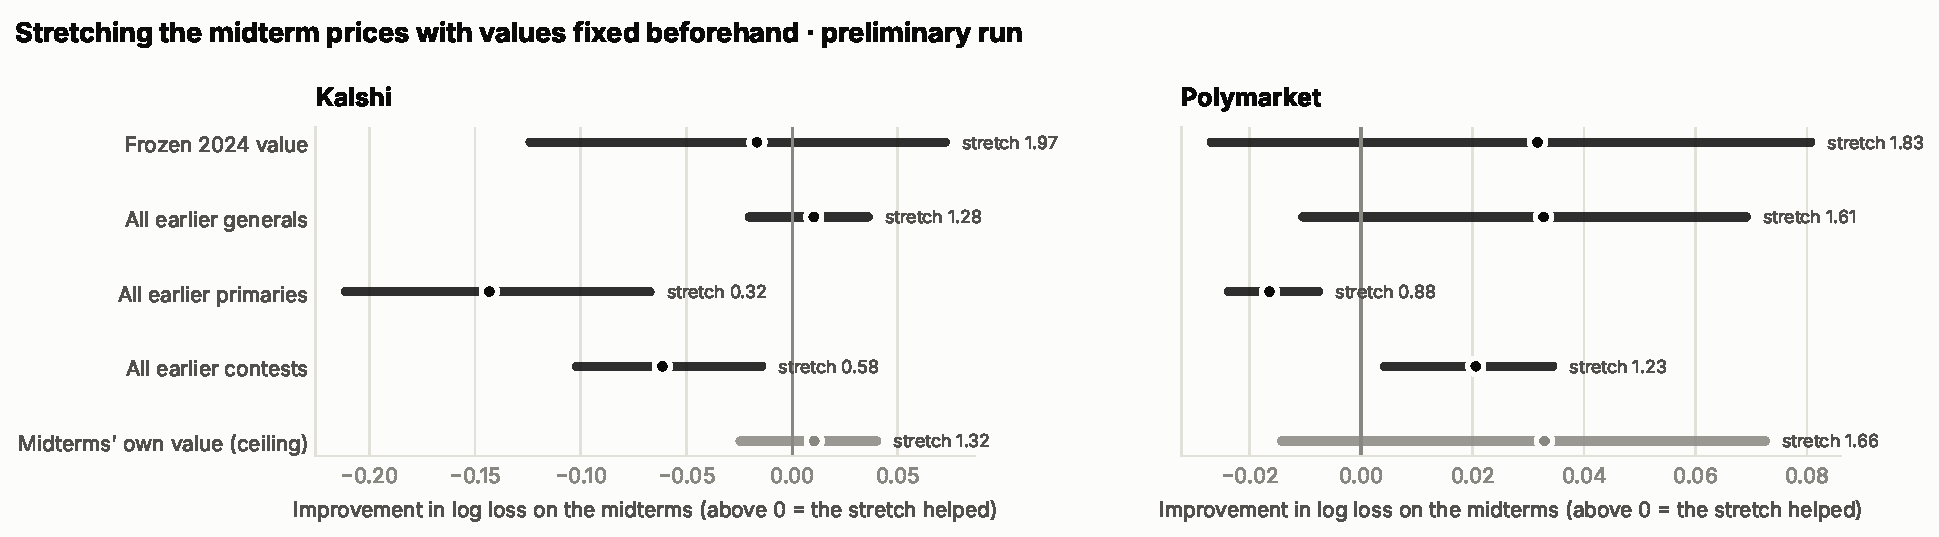
\includegraphics[width=\textwidth]{figures/cmp_scores.pdf}
\caption{Improvement in the log loss of the midterm prices when each is stretched by a value fixed before the vote.
Above zero, the stretch helped. Intervals resample states with the stretch held fixed. The last row uses the midterms'
own stretch and marks the best any single value could have done.}\label{fig:scores}
\end{figure}

\paragraph{How strong is the evidence?}
Table~\ref{tab:pvalues} gives p-values for the two questions, computed naively and allowing for contests in one state
moving together (the column headed ``$p$, states''). Allowing for states matters a great deal. On Polymarket, the midterm stretch is clearly above 1 either
way ($p = 0.02$ allowing for states; 0.2\% of state resamples at or below 1). On Kalshi it is not ($p = 0.15$).
Persistence is weaker. Stretching Polymarket's midterm prices by the 2024 value made the results about 99 times as
likely as the raw prices did, which looks decisive if contests are treated as independent, but gives $p = 0.13$ once
states are allowed to move together. With the value from all earlier general elections, $p = 0.06$. A single election
night of about 35 states cannot establish persistence on its own.

\begin{table}[tbp]
\centering\small
\caption{Exploratory p-values, one-sided. Level: is the midterm stretch above 1? Persistence: does a stretch fixed
before the vote make the midterm results more likely than the raw prices do? ``Times as likely'' is the ratio of the
two likelihoods. ``${\le}\,1$'' is the share of the test's state resamples at or below 1. ``$p$, states'' allows for contests
in one state moving together.}\label{tab:pvalues}
\setlength{\tabcolsep}{4.5pt}
\begin{tabular}{llrrrr}
\toprule
 & Question & ${\le}\,1$ & Times as likely & Naive $p$ & $p$, states \\
\midrule
Kalshi & Level & 7.9\% & & 0.024 & 0.153 \\
 & Persistence, 2024 value (1.97) & & 0.04 & 0.750 & 0.622 \\
 & Persistence, earlier generals (1.28) & & 6.8 & 0.073 & 0.235 \\
\midrule
Polymarket & Level & 0.2\% & & 0.001 & 0.022 \\
 & Persistence, 2024 value (1.83) & & 98.6 & 0.044 & 0.133 \\
 & Persistence, earlier generals (1.61) & & 115.5 & 0.008 & 0.062 \\
\bottomrule
\end{tabular}
\end{table}

\subsection{Summary}

General-election markets on both platforms were underconfident in 2024 and, on the races both platforms listed,
equally underconfident in the 2026 midterms. Polymarket passed the pre-registered test; Kalshi's result is inconclusive,
because the low-profile races only Kalshi listed went the other way. Kalshi's primaries were strongly overconfident in
the training data, a result not explained by runoffs or late settlement, and corrections learned from primaries made
midterm prices worse. The pattern is consistent with primaries being traded differently from general elections, and
not with the underconfidence having faded over time.

\section{Backtest}\label{sec:backtest}

If general-election favourites are underpriced, buying them should have paid. This section checks that looking
backwards, on the two general-election nights in the data: 5 November 2024 and the midterms of 3 November 2026. It was
not part of the pre-registration, every rule in it was chosen after seeing the results, and it is included for
discussion rather than as evidence.

\paragraph{What a bet is.} \$100 on the favourite of every US contest with a usable price at the snapshot, held until
the market settled. On Kalshi a bet costs the actual asking price at the snapshot plus the taker fee of 7\% of the price
times one minus the price. On Polymarket only a recorded price is available, so buying is assumed to cost 1 cent more,
plus the taker fee of 4\% of the price times one minus the price from 30 March 2026; there was no fee in 2024. Unlike
Sections~\ref{sec:data} to~\ref{sec:results}, the bets include favourites priced above 95\% and contests in Georgia,
Louisiana and Mississippi, since those bets still settle. That gives 97 bets on Kalshi and 91 on Polymarket in 2024,
and 547 and 419 on the midterms. Intervals resample states, as in Section~\ref{sec:results}.

\subsection{Buying every favourite earns little}

Buying every favourite returned 0.9\% per bet on Kalshi's midterms and 3.0\% on Polymarket's, after costs, and both
intervals include zero (Table~\ref{tab:backtest}). In 2024 the returns were 3.5\% on Kalshi and 7.3\% on Polymarket;
the Polymarket figure benefits from a night on which only 3 of 91 favourites lost, and from the absence of fees.

Two things eat the profit (Figure~\ref{fig:bt_bands}). Close races, with favourites priced between 50\% and 70\%, lost
money on the midterms: 16.5\% on Kalshi's 48 bets and 3.8\% on Polymarket's 34. This matches Section~\ref{sec:results},
where close races were priced about right and the underconfidence sat in clear favourites. Costs are also heaviest
there: Kalshi's fee is about 3\% of the price for a 60\% favourite and under 1\% for a 90\% favourite. At the other end,
favourites priced above 95\% almost always won, but each win paid only 1 to 2 cents on the dollar.

\begin{table}[!htbp]
\centering\small\setlength{\tabcolsep}{4.5pt}
\caption{The backtest: \$100 on every favourite of a group, after costs. Return is profit per \$100 staked, with a 95\%
interval from resampling states. When every bet in a group won, the interval cannot reach below zero, however few the
bets. The last row of each platform takes the best price window of 2024 (Figure~\ref{fig:bt_windows}) and applies it to
the midterms.}\label{tab:backtest}
\begin{tabular}{llL{2.9cm}rrrlr}
\toprule
 & Night & Rule & Bets & Upsets & Return, \% & 95\% interval & Profit \\
\midrule
Kalshi & 2024 & Every favourite & 97 & 12 & $+3.5$ & $-5.9$ to $+12.8$ & \$339 \\
 & & At or above 70\% & 68 & 1 & $+5.9$ & $+1.5$ to $+9.0$ & \$400 \\
 & & 85--90\% & 6 & 0 & $+11.7$ & $+10.6$ to $+12.7$ & \$70 \\
\addlinespace
 & Midterms & Every favourite & 547 & 36 & $+0.9$ & $-3.5$ to $+5.0$ & \$481 \\
 & & At or above 70\% & 499 & 13 & $+2.6$ & $-0.4$ to $+5.0$ & \$1{,}275 \\
 & & 85--90\% & 29 & 1 & $+8.0$ & $-0.1$ to $+12.5$ & \$232 \\
 & & 2024's best window, 75--85\% & 47 & 8 & $+0.5$ & $-27.3$ to $+20.5$ & \$24 \\
\midrule
Polymarket & 2024 & Every favourite & 91 & 3 & $+7.3$ & $+1.5$ to $+12.9$ & \$663 \\
 & & At or above 70\% & 81 & 2 & $+2.9$ & $-3.3$ to $+7.0$ & \$234 \\
 & & 85--90\% & 6 & 0 & $+11.8$ & $+10.5$ to $+12.9$ & \$71 \\
\addlinespace
 & Midterms & Every favourite & 419 & 20 & $+3.0$ & $-0.7$ to $+6.6$ & \$1{,}256 \\
 & & At or above 70\% & 385 & 6 & $+3.6$ & $+1.6$ to $+5.5$ & \$1{,}386 \\
 & & 85--90\% & 26 & 1 & $+8.1$ & $-0.3$ to $+12.9$ & \$211 \\
 & & 2024's best window, 60--70\% & 15 & 6 & $-10.9$ & $-53.8$ to $+36.8$ & $-\$164$ \\
\bottomrule
\end{tabular}
\end{table}

\begin{figure}[!htbp]
\centering
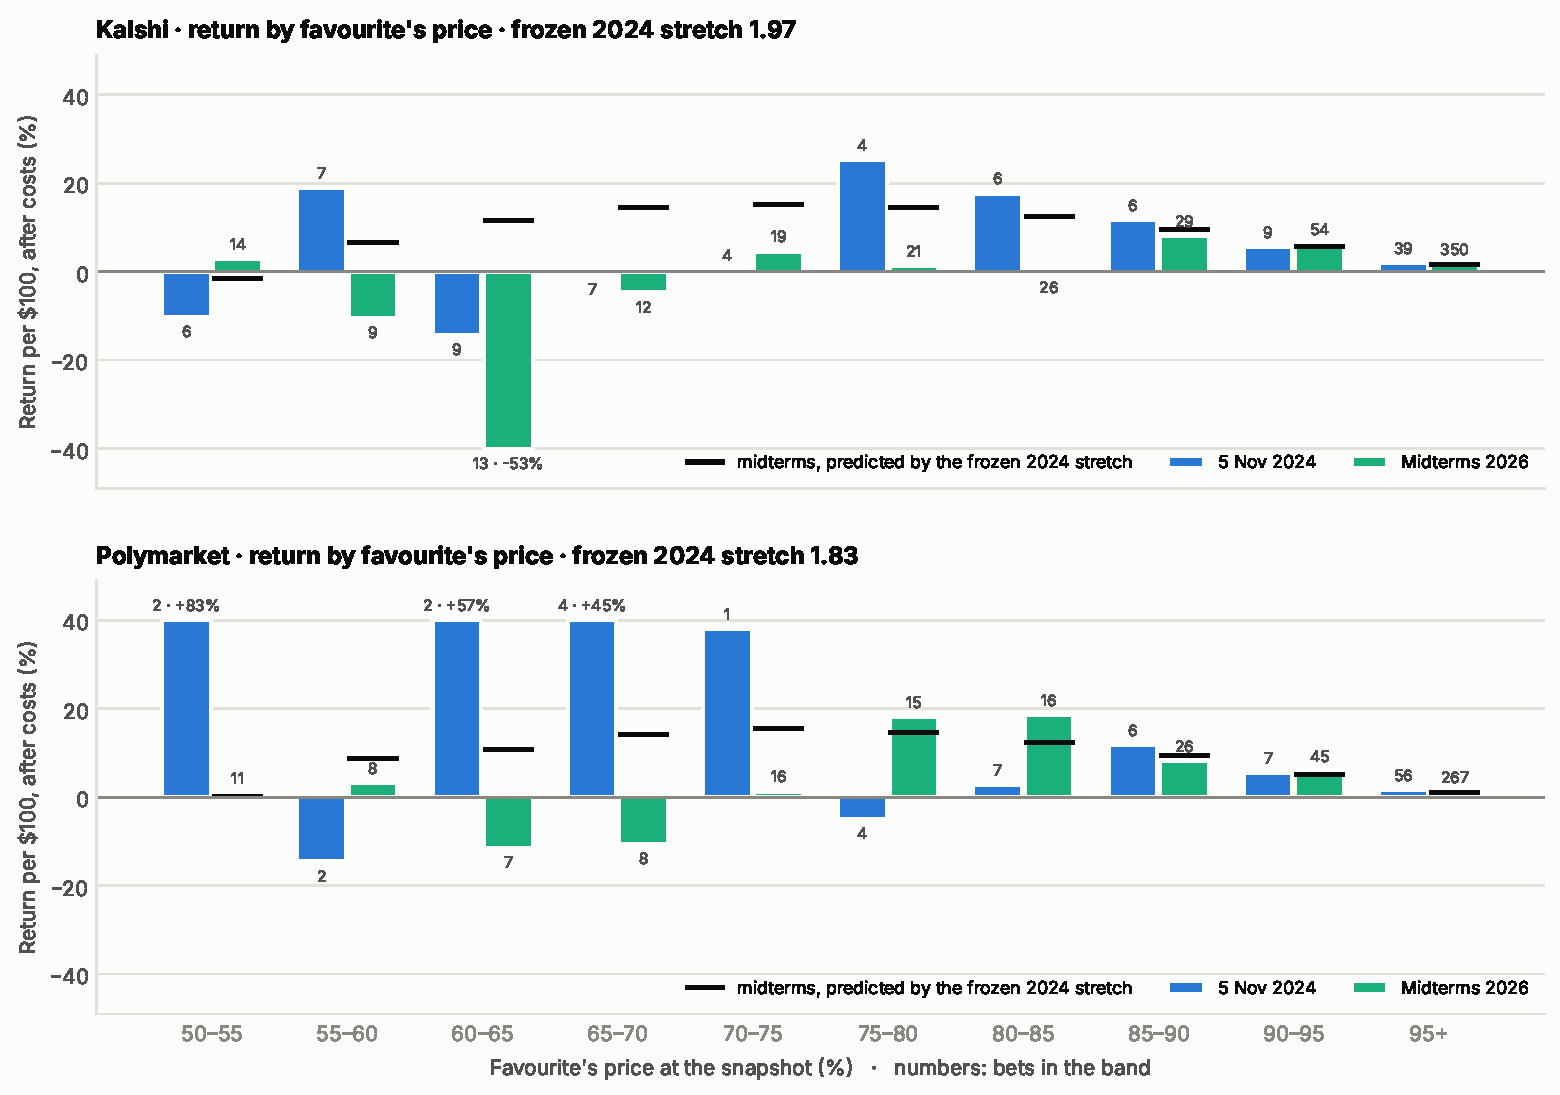
\includegraphics[width=0.9\textwidth]{figures/bt_bands.pdf}
\caption{Return per \$100 after costs, by the favourite's price, on 5 November 2024 (blue) and the midterms (green).
Numbers give the bets in each band; bars beyond $\pm 40\%$ are cut and their value written out. Black marks: the return
the frozen 2024 stretch predicted for the midterm bets in each band, given the prices actually paid. That stretch was
fixed before the vote, so for the midterms the marks are a genuine forecast.}\label{fig:bt_bands}
\end{figure}

\subsection{Favourites above 70\%}

Leaving out the close races fixes most of this. Figure~\ref{fig:bt_thresholds} applies the rule ``buy every favourite
priced at or above a threshold'' for every threshold from 50\% to 95\%. Raising the threshold drops the close races
that lost money, but it also drops bets, and the bets that remain are expensive, with less room to pay. Total profit
therefore peaks in between, and on three of the four platform-nights it peaks close to 70\%: at 71\% on Kalshi's
midterms (\$1{,}401 on 495 bets), at 68\% on Polymarket's midterms (\$1{,}410 on 389) and at 68\% on Kalshi in 2024
(\$596 on 73). At exactly 70\%, the rule returned 2.6\% per bet on Kalshi's midterms and 3.6\% on Polymarket's, the
latter with an interval wholly above zero (1.6\% to 5.5\%). The exception is Polymarket in 2024, where nine of the ten
favourites priced between 50\% and 70\% won, so the most profitable rule was to buy everything.

This is what the bias found in Section~\ref{sec:results} would lead one to expect. A stretch above 1 says favourites
win more often than their prices imply. The gap is zero at 50\%, where the stretch changes nothing, and shrinks again
towards 100\%, where there is no room left. The black marks in Figure~\ref{fig:bt_bands} show the returns the frozen
2024 stretch predicted for the midterm bets. Above 85\%, they are close to what happened: on Kalshi 9.6\% predicted
against 8.0\% earned between 85\% and 90\%, and 5.7\% against 6.3\% between 90\% and 95\%; Polymarket is similar.
Between 60\% and 85\%, the stretch predicted returns of 10\% to 15\%. Kalshi's midterm favourites earned at most
5\% in any of those bands and lost heavily between 60\% and 65\%; Polymarket's fell short of the prediction between
60\% and 75\% and beat it between 75\% and 85\%. A single stretch describes clear favourites well and overstates the
edge in moderately close races.

The margins are thin. Over a whole night, buying every favourite above 70\% returned 2\% to 4\% per bet on the
midterms, and Kalshi's 2024 markets settled only in January 2025, tying the money up for about two months.

\begin{figure}[!htbp]
\centering
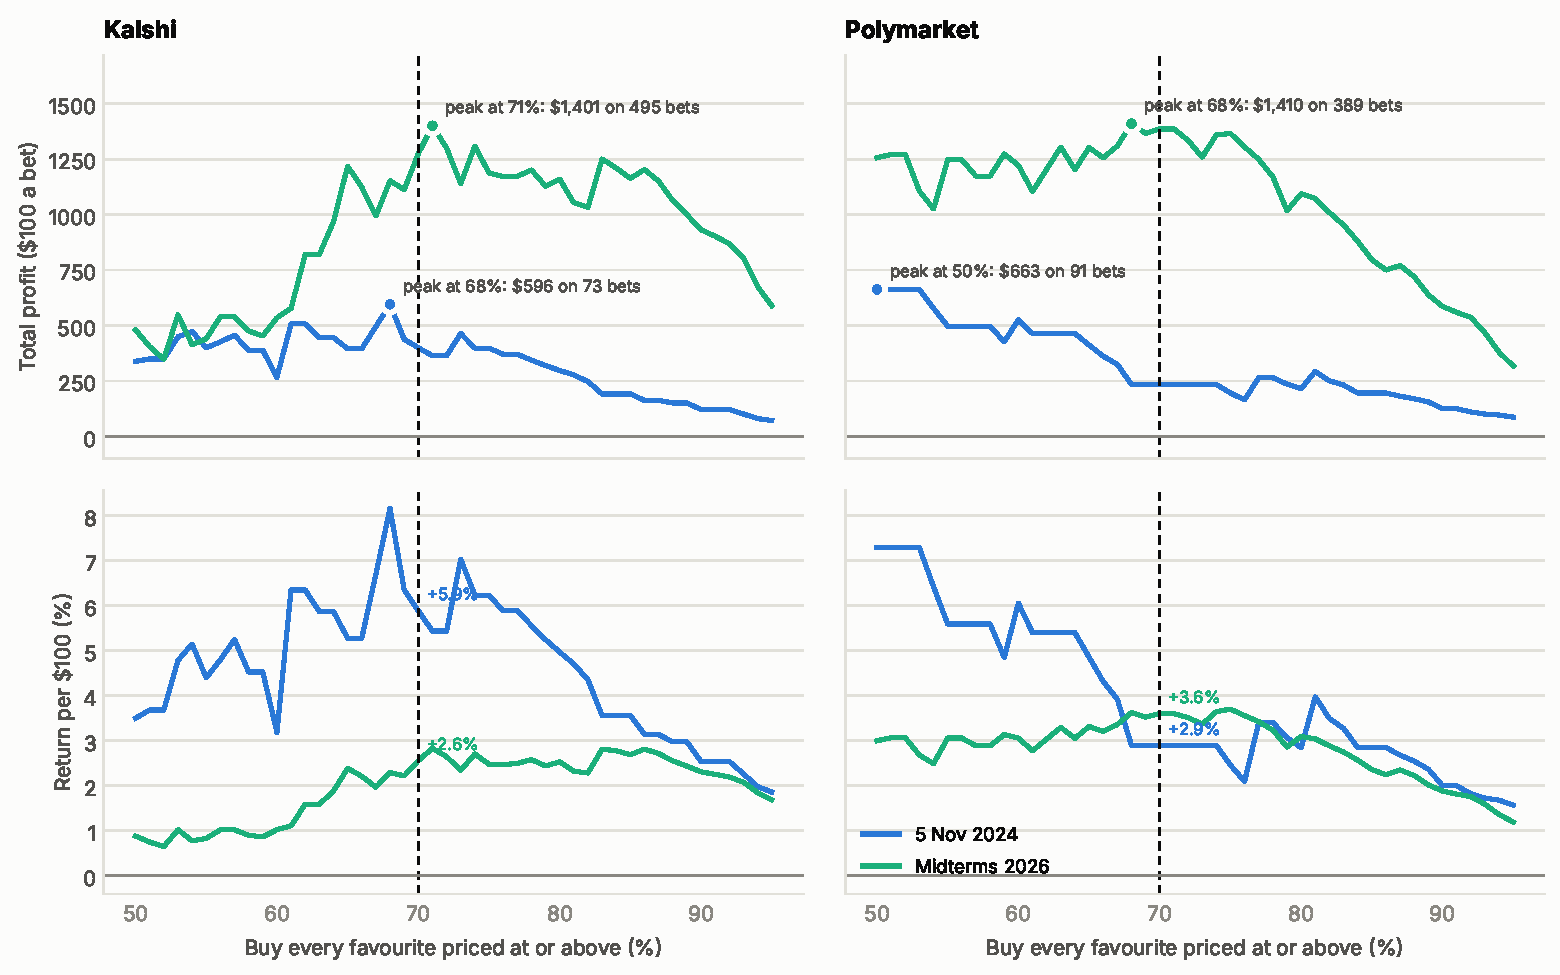
\includegraphics[width=0.86\textwidth]{figures/bt_thresholds.pdf}
\caption{Buying every favourite priced at or above a threshold, for thresholds from 50\% to 95\% in steps of one point.
Top: total profit at \$100 a bet, with each night's peak marked. Bottom: return per \$100. Dashed line: 70\%. The
jagged lines show how much a single upset moves the result.}\label{fig:bt_thresholds}
\end{figure}

\subsection{The 85--90\% band, and why it is probably overfitted}

The best-paying band that made money on both nights and on both platforms is 85\% to 90\%. Favourites priced there
returned 11.7\% on Kalshi and 11.8\% on Polymarket in 2024, and 8.0\% and 8.1\% on the midterms. Only 2 of their 67
bets lost.

It would be a mistake to read this as a strategy. There are few bets: six on each platform in 2024, where one more
upset would have turned the profit into a loss, and 29 and 26 on the midterms, where the intervals reach below zero.
The 2024 intervals look narrow only because every bet won, and resampling bets that all won can never produce a loss.
Nothing in the bias singles out this band either: the frozen stretch predicted larger returns between 65\% and 85\%
than between 85\% and 90\% (Figure~\ref{fig:bt_bands}).

More importantly, the band was found by searching. Figure~\ref{fig:bt_windows} shows every price window with edges at
5-point steps, 55 of them per platform and night. With that many to choose from, some window will look excellent on any
night, and which one it is changes from night to night: 75--85\% for Kalshi in 2024 (21\% on 10 bets), 85--90\% for
Kalshi's midterms, 60--70\% for Polymarket in 2024 (49\% on 6 bets) and 80--85\% for Polymarket's midterms (19\% on 16
bets). A trader who had picked the best window of 2024 and bought it on the midterms would have made 0.5\% on Kalshi and
lost 10.9\% on Polymarket (Table~\ref{tab:backtest}). Every strategy looks good in a backtest once it has been adjusted
enough, and the 85--90\% band was chosen by looking at the same two nights on which it is evaluated.

\begin{figure}[!htbp]
\centering
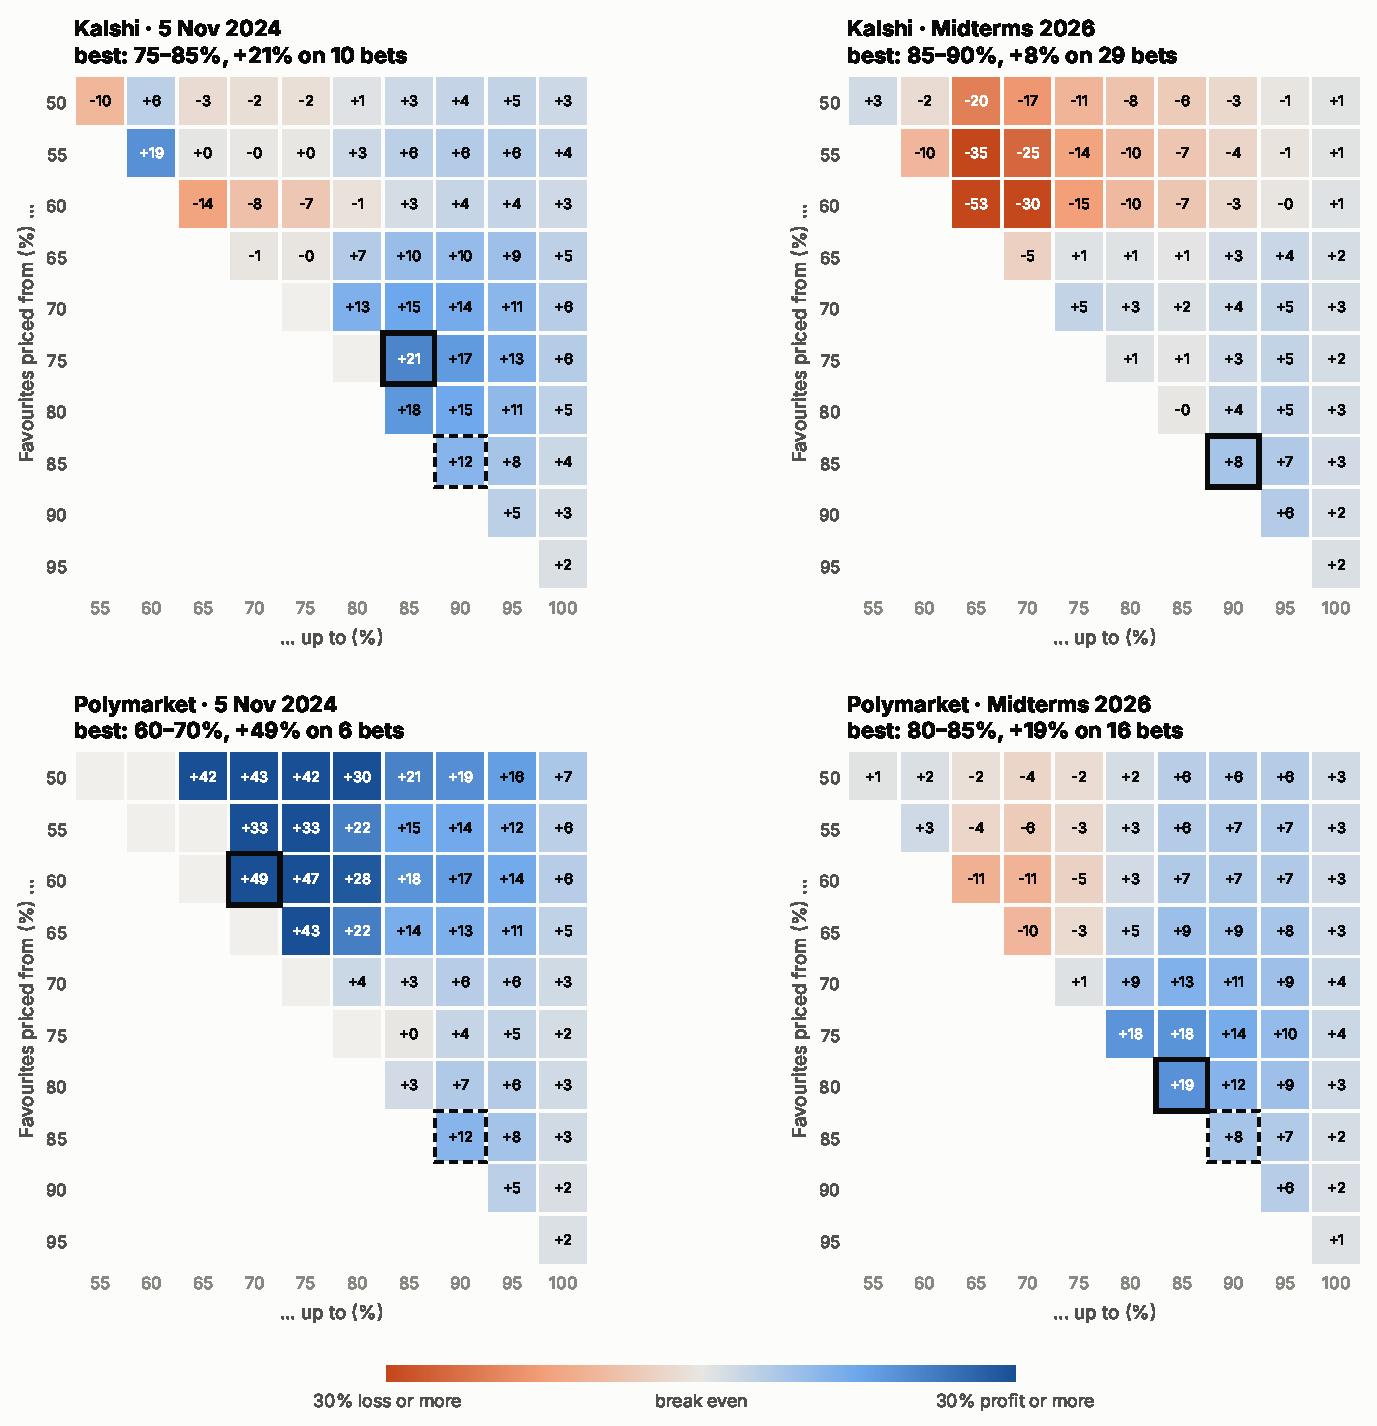
\includegraphics[width=0.8\textwidth]{figures/bt_windows.pdf}
\caption{Every price window: buy every favourite priced from the row's value up to the column's value (the last column
includes everything up to 100\%). Colour and number: return per \$100 after costs. Blank: fewer than five bets. Solid
outline: the best window on that night. Dashed outline: 85--90\% (on Kalshi's midterms the two coincide).}
\label{fig:bt_windows}
\end{figure}

\subsection{What the backtest can and cannot say}

Beyond the search problem, the results flatter the strategy in several ways. Contests enter only if they settled with
one of the two listed candidates winning, and the 40 midterm races still unsettled lean towards those in which the
favourite struggled. Bets on one night are not independent: a national swing moves every race at once, and resampling
states does not capture that, so the two nights are in effect two observations. The Kalshi asking price is good only
for the first few contracts, and the depth of the order book behind it was not recorded. No interest is counted on the
money tied up until settlement.

What the backtest does support is the shape of the opportunity, if the underconfidence persists: the money is in clear
favourites rather than in close races, it fades above 95\%, and after costs it is a few percent per bet. Whether a rule
such as ``buy every favourite above 70\%'' works can only be settled the way the main hypothesis was: by fixing it
before the next general election and checking it afterwards.

\section{Deviations and limitations}\label{sec:limitations}

\subsection{Deviations from the pre-registration}

\paragraph{Code written after the vote.} Collecting the settled midterm markets needed code that did not exist before
the vote: a script to download them, one to clean them, and an option in the pricing scripts that prices the midterm
contests and appends them to the price table. The rules applied are the frozen ones, and every earlier row of the price
table is unchanged byte for byte. The test's own safeguard confirms this: before running, it recomputed both 2024
values from the table and found them unchanged.

\paragraph{Polymarket trade records.} On 24 October 2026, after the freeze, Polymarket retired the interface that served
past trades. For the midterms, the rule ``drop the contest if neither candidate traded in the day before the snapshot''
therefore reads the trades from its replacement. The rule is unchanged, and the training prices, collected before the
change, were not recomputed.

\paragraph{A fault in the fitting routine.} After the vote we found that the frozen routine, Newton's method started at
a stretch of 1 and limited to $\pm 50$, can overshoot and stop at $+50$ when the best stretch is below zero, that is,
when more favourites lost than their prices allowed for. We refitted every frozen interval with a routine that always
finds the maximum. Two intervals change, both for Kalshi and both from resampling election days: all training contests
go from 0.14--1.03 to 0.14--1.02, and primaries from 0.03--0.70 to 0.01--0.69. The point estimates, the 2024 values,
every interval from resampling states (including the midterm test) and every Polymarket interval are unchanged. The
archived code is left as it was. The corrected values are given beside the frozen ones (Table~\ref{tab:training}), and
the exploratory checks of Figure~\ref{fig:primary_checks} use the corrected routine. An exploratory table in the
repository that lists a stretch for each election day shows 50 or 15.8 for four Kalshi primary days, whose true values
lie between $-0.92$ and 0.

\paragraph{Analyses added after the vote.} Only the main hypothesis and its test were fixed in advance. The forecast
scores, the comparison of races listed on both platforms, the p-values, the checks on the training primaries and the
backtest (Sections~\ref{sec:exploratory} and~\ref{sec:backtest}) were all designed after the results were known, and
are reported as exploratory.

\subsection{Limitations}

\paragraph{One night, few independent pieces of information.} The test rests on a single election night and about 35
states per platform. Resampling states allows for races within a state moving together, but not for a polling miss that
moves every state at once. Across the whole study there are only two general-election nights of any size. Persistence
is the weakest link: allowing for states, the evidence that the 2024 value improves midterm prices is far from
conclusive ($p = 0.13$ on Polymarket).

\paragraph{The primary result is untested.} Kalshi's overconfidence in primaries comes from 78 contests on 21 days,
most of them in 2026, and was found in the data rather than tested. The midterms contain no primaries and say nothing
about it.

\paragraph{Which contests enter.} A contest enters only if it settled with one of its two listed candidates winning, and
races with more than two serious candidates are left out. In this preliminary run, the 40 midterm races still unsettled
lean towards those in which the favourite struggled, which tilts the results towards underconfidence; the reading is
judged on the final run. Favourites priced above 95\%, the majority of contests, are excluded by design, so the results
describe races with real uncertainty on election day.

\paragraph{One price per contest.} Each contest is priced once, at least an hour before the first polls close. A Kalshi
midpoint can be stale when the order book is thin, and a Polymarket recorded price is not a quote anyone could trade at.
Dropping the Kalshi contests in which neither candidate traded in the day before changes little, but price noise
cannot be ruled out.

\paragraph{One number per group.} The stretch assumes the same distortion at every price. Sections~\ref{sec:results}
and~\ref{sec:backtest} show that close races and clear favourites behaved differently on the midterms, so a single
stretch summarises a group but overstates the edge in close races.

\paragraph{Two platforms in a changing market.} The platforms listed different races, and between 2023 and 2026 both
grew quickly and changed regulatory status. Patterns found in this period may weaken as the markets mature, and need
not hold for other countries or other kinds of event.

\section{Discussion}\label{sec:discussion}

\paragraph{A familiar bias, not yet a persistent one.} The simplest reading of the general-election results is that
election markets show the favourite--longshot bias long documented in racetrack and sports betting
\citep{griffith1949,thaler1988,snowberg2010}: favourites are priced too cheaply and long shots too dearly. We cannot yet
establish it as a persistent feature of election markets. The evidence rests on two general-election nights, 2024 and
2026, and two nights that point the same way may still be a coincidence; allowing for states moving together, the
direct test of persistence is not significant ($p = 0.13$ on Polymarket). US general elections come only every two
years, so settling the question needs a much longer record. Primaries also do not fit the pattern. Kalshi's primaries
were strongly overconfident, the opposite of the betting-market bias, and they trade far less than general elections
(Section~\ref{sec:data}). Whatever drives the bias, it seems to depend on the kind of race and who trades it, not only
on the market being a betting market.

\paragraph{Information and hedging rather than profit.} Even if the bias persists, little is left after costs: buying
favourites above 70\% earned a few percent per bet on the midterms, and the more profitable rules were found by
searching the same nights on which they were judged (Section~\ref{sec:backtest}). The greater value of these markets
probably lies elsewhere. Their prices are fast, public forecasts that have rivalled polls
\citep{berg2008,rothschild2009}, and the results here hint that a small correction learned from past general elections can make
them slightly more accurate. Their contracts also let investors hedge exposure to an event directly, such as a holding in a solar-energy
fund before the 2024 presidential election; such hedges look practical for small positions, though thin liquidity
limits them at institutional scale \citep{kirillov2026hedge}.

\paragraph{Rules shape who trades.} Regulation and politics decide which venue attracts which traders, which contracts
can be listed at all, and which markets draw volume. Kalshi could list US election contracts only after winning its
case against the CFTC in 2024; Polymarket blocked US users for most of the period studied and re-entered the US market
in 2025 (Section~\ref{sec:data}). The calibration measured here belongs to that particular period of fast growth and
changing rules. A new US administration, or a change in how regulators treat election contracts, could alter who trades
on each platform, which races are listed and how heavily each is traded, and with them the patterns reported in this
paper.

\section{Conclusion}\label{sec:conclusion}

Favourites in US general-election markets were underpriced again in the 2026 midterms. On Polymarket, the
pre-registered test found the markets underconfident and consistent with 2024 (a stretch of 1.66, interval 1.21 to
2.91). Kalshi's test was inconclusive (1.32, 0.88 to 2.35), but on the 141 races both platforms listed, the two were
equally underconfident (1.68 and 1.65), and Kalshi's weaker overall result comes from the down-ballot races that only it
listed. This is the same direction as the favourite--longshot bias documented in betting markets for more than seventy
years \citep{griffith1949,thaler1988,snowberg2010}: favourites win more often than their prices say. Stretching the
midterm prices by the value learned from earlier general elections made them slightly more accurate on both platforms,
though not by enough to rule out chance.

Primaries were different. Kalshi's primary favourites won far less often than priced (a stretch of 0.32), the result is
not explained by runoffs or late settlement, and a correction learned from primaries made the midterm prices worse. This
was found in the data rather than tested, and the 2028 primary season is the place to test it, fixed in advance in the
same way.

Whether the underpricing of favourites can be traded is a separate question, and two general-election nights cannot
answer it. Buying every favourite above 70\% earned 2.6\% to 3.6\% per bet on the midterms after costs. But the most
profitable rules were found by searching the same two nights on which they were judged, and the best rule of 2024 did
not carry over to 2026. A rule fixed before the 2028 general election would be a fair test.

This version reports the preliminary run. The final run, due by 31 January 2027, decides the pre-registered reading.

\section*{Data and code availability}

The code, the training results and the midterm test as frozen before the vote are archived on Zenodo
\citep{kirillov2026code}, and the raw market data in a separate archive \citep{kirillov2026data}. The code written
after the vote, the midterm data and the notebooks that produce every figure and table in this paper are in the
study's public repository, \url{https://github.com/nickdatak/prediction-markets-overconfident-underconfident}.

\section*{Use of AI tools}

Claude (Anthropic), an AI assistant, was used to help write the analysis code and to draft and edit the text. The
author directed the study, checked the analyses and is responsible for the content.


\bibliographystyle{plainnat}
\bibliography{references}

\end{document}
